\documentclass[12pt,a4paper]{report}
\usepackage[utf8]{inputenc}
\usepackage{amsfonts}
\usepackage{setspace}
\usepackage{graphicx}
\usepackage{array}
\usepackage{fancyhdr}
\usepackage{geometry}
\usepackage{ragged2e}
\usepackage{color}
\usepackage[backend=biber, sorting=none, style=ieee]{biblatex}
\usepackage{float}

\addbibresource{reference.bib}

\geometry{
a4paper,
total={210mm,297mm},
left=1.15in,
right=0.85in,
top=1.0in,
bottom=1.0in,
}
\begin{document}
\pagestyle{empty}
\begin{center}

{\large \textbf{Visvesvaraya Technological University, Belagavi – 590018}}
\begin{figure}[hbtp]
\centering

\includegraphics[width=2.3cm,height=2.8cm]{./pic/vtu}
\end{figure}

\textbf{PROJECT REPORT}
\par
\textbf{ON}
\par
\vspace{6pt}
{\Large \textbf{CLOUD-BASED SMART MONITORING SYSTEM
FOR BABY HEALTH AND SAFETY}}
\par
\vspace{12pt}
\par
\textit{\textbf{Submitted in partial fulfillment for the award of degree of }}
\par
\vspace{12pt}
\large \textbf{BACHELOR OF ENGINEERING }
\par
\textbf{in}
\par
\large \textbf{COMPUTER SCIENCE \& ENGINEERING}
\par
\vspace{12pt}
\textit{\textbf{Submitted by}}
\vspace{8pt}

% \textbf{\large Aaron Tauro}\qquad \qquad \qquad \qquad \textbf{\large 4SO21CS002}\\ \vspace{3pt} 
% \textbf{\large Abhik L Salian}\qquad \qquad \qquad \qquad \textbf{\large 4SO21CS004}\\ \vspace{3pt}
% \textbf{\large Akhil Shetty M}\qquad \qquad \qquad \qquad \textbf{\large 4SO21CS013}\\ \vspace{3pt}
% \textbf{\large H Karthik P Nayak}\qquad \qquad \qquad \qquad \textbf{\large 4SO21CS058}\\ \vspace{3pt}
\begin{center}
    \begin{tabular}{l@{\hspace{2cm}}r}
      \textbf{\large Aaron Tauro}       & \textbf{4SO21CS002} \\
      \textbf{\large Abhik L Salian}    & \textbf{4SO21CS004} \\
      \textbf{\large Akhil Shetty M}    & \textbf{4SO21CS013} \\
      \textbf{\large H Karthik P Nayak} & \textbf{4SO21CS058} \\
    \end{tabular}
  \end{center}
\vspace{12pt}
\textit{\textbf{Under the Guidance of}}
\par
\vspace{6pt}
\textbf{Dr Sridevi Saralaya}
\par
\vspace{2pt}
\normalsize { Professor, Department of CSE }
\par
\begin{figure}[hbtp]
\centering

\includegraphics[scale=0.5]{./pic/sjeclogo}
\end{figure}
\large \textbf{DEPT. OF COMPUTER SCIENCE AND ENGINEERING}
\par \Large \textbf{ST JOSEPH ENGINEERING COLLEGE}
\par 
\textbf{An Autonomous Institution}
\par
{\large{(Affiliated to VTU Belagavi, Recognized by AICTE, Accredited by NBA)}}
\par
\vspace{3pt}
{\large \textbf{Vamanjoor, Mangaluru - 575028, Karnataka}}
\par 
\vspace{12pt}
{\Large \textbf{2024-25}}
\end{center}
\newpage


% Certificate Page
\begin{center}
\LARGE \textbf{ST JOSEPH ENGINEERING COLLEGE}
\par
\Large \textbf{An Autonomous Institution}
\par \large{(Affiliated to VTU Belagavi, Recognized by AICTE, Accredited by NBA)}
\par \vspace{3pt}
\large \textbf{Vamanjoor, Mangaluru - 575028, Karnataka}
\par \vspace{12pt}  
\par
\large \textbf{DEPT. OF COMPUTER SCIENCE AND ENGINEERING}
\par
\begin{figure}[hbtp]
\centering

\includegraphics[scale=0.5]{./pic/sjeclogo}
\end{figure}


{\Large \textbf{CERTIFICATE}}
\end{center}
\justifying
\par
\setstretch{1.2}
\noindent 
Certified that the project work entitled \textbf{"Cloud-Based Smart Monitoring System
for Baby Health and Safety"} carried out by\vspace{0.25in} 
\par

\noindent 
% \vspace{2pt} 
% \textbf{\large \quad \quad \qquad Student Name 1}\qquad \qquad \qquad \qquad \textbf{\large 4SO20CS001}\\ \vspace{2pt} 
% \textbf{\large \quad \quad \qquad Student Name 2}\qquad \qquad \qquad \qquad \textbf{\large 4SO20CS002}\\ \vspace{2pt}
% \textbf{\large \quad \quad \qquad Student Name 3}\qquad \qquad \qquad \qquad \textbf{\large 4SO20CS003}\\ \vspace{2pt}
% \textbf{\large \quad \quad \qquad Student Name 4}\qquad \qquad \qquad \qquad \textbf{\large 4SO20CS004}\\ \vspace{1pt}
\begin{center}
    \begin{tabular}{l@{\hspace{2cm}}r}
      \textbf{\large Aaron Tauro}       & \textbf{4SO21CS002} \\
      \textbf{\large Abhik L Salian}    & \textbf{4SO21CS004} \\
      \textbf{\large Akhil Shetty M}    & \textbf{4SO21CS013} \\
      \textbf{\large H Karthik P Nayak} & \textbf{4SO21CS058} \\
    \end{tabular}
  \end{center}
\justifying

\noindent
the bonafide students of VII semester Computer Science \& Engineering in partial fulfillment for the award of Bachelor of Engineering in Computer Science and Engineering of the Visvesvaraya Technological University, Belagavi during the year 2024-2025. It is certified that all corrections/suggestions indicated during Internal Assessment have been incorporated in the report. The project report has been approved as it satisfies the academic requirements in respect of project work prescribed for the said degree. 

\par
\vspace{0.33in}
\setstretch{1.15}
\begin{tabbing}
---------------------------------\hspace{0.3in}\=----------------------------------- \hspace{0.3in}\=--------------------------------- \\
\textbf{Dr Sridevi Saralaya}\>\hspace{0.3in}\textbf{Dr Sridevi Saralaya }\>\hspace{0.3in}\textbf{Dr Rio D'Souza}\\
\hspace{0.5in}Project Guide\>\hspace{0.50in} HOD-CSE \>\hspace{0.6in}Principal
\end{tabbing}

\begin{center}
\large \textbf{External Viva}:
\end{center}
\begin{flushleft}
\begin{normalsize}Examiner's Name \end{normalsize}
\hspace{6.5cm}
\begin{normalsize}Signature with Date\end{normalsize}
\end{flushleft}
\vspace{0.1in}
\begin{flushleft}
1. \ldots\ldots\ldots\ldots\ldots\ldots \ldots \hspace{5.8cm}\ldots\ldots\ldots\ldots \ldots\ldots\ldots 
\par
\vspace{0.2in}	
2. \ldots\ldots\ldots\ldots\ldots\ldots \ldots \hspace{5.8cm}\ldots\ldots\ldots\ldots \ldots\ldots\ldots 
\end{flushleft}
\newpage

% Declaration Page
\centering
\LARGE \textbf{ST JOSEPH ENGINEERING COLLEGE}
\par
\Large \textbf{An Autonomous Institution}
\par \large{(Affiliated to VTU Belagavi, Recognized by AICTE, Accredited by NBA)}
\par \vspace{3pt}
\large \textbf{Vamanjoor, Mangaluru - 575028, Karnataka}
\par \vspace{12pt}  
\par
\large \textbf{DEPT. OF COMPUTER SCIENCE AND ENGINEERING}
\par
\begin{figure}[hbtp]
\centering

\includegraphics[scale=0.5]{./pic/sjeclogo}
\end{figure}

\begin{center}
{\Large \textbf{DECLARATION}}
\end{center}
\justifying
\par
\setstretch{1.5}
\noindent We hereby declare that the entire work embodied in this Project Report titled
\textbf{``Cloud-Based Smart Monitoring System for Baby Health
and Safety''} has been carried out by us at St Joseph Engineering College, Mangaluru under the supervision of \textbf{Dr Sridevi Saralaya,} for the award of \textbf{Bachelor of Engineering} in \textbf{Computer Science \& Engineering}. This report has not been submitted to this or any other University  for the award of any  other degree. \\
\vspace{0.25in}

\setstretch{1.75}
\begin{flushleft}
\textbf{Aaron Tauro  USN:4SO21CS002}\\
\vspace{0.1in}
\textbf{Abhik L Salian  USN:4SO21CS004}\\
\vspace{0.1in}
\textbf{Akhil Shetty M  USN:4SO21CS013}\\
\vspace{0.1in}
\textbf{H Karthik P Nayak  USN:4SO21CS058}\\
\end{flushleft}

% \newpage
\setstretch{1.2}
\chapter*{\centering Acknowledgement}
\addcontentsline{toc}{chapter}{\numberline{}Acknowledgement}
We dedicate this page to acknowledge and thank those responsible for the shaping of the project. Without their guidance and help, the experience while constructing the dissertation would not have been so smooth and efficient.
\par
\vspace{0.15in}
\noindent We sincerely thank our Project guide \textbf{Dr Sridevi Saralaya}, Professor, Computer Science and Engineering for her guidance and valuable suggestions which helped us to complete this project. We also thank our Project coordinators \textbf{Ms Supriya Salian} and \textbf{Dr Saumya Y M},  Dept of CSE, for their consistant encouragement. 
\par
\vspace{0.15in}
\noindent We owe a profound gratitude to \textbf{Dr Sridevi Saralaya}, Head of the Department, Computer Science and Engineering, whose kind support and guidance helped us to complete this work successfully
\par
\vspace{0.15in}
\noindent We are extremely thankful to our Principal, \textbf{Dr Rio D’Souza}, Director,  \textbf{Rev. Fr Wilfred Prakash D'Souza}, and Assistant Director, \textbf{Rev. Fr Kenneth Rayner Crasta} for their support and encouragement.
\par
\vspace{0.15in}
\noindent We would like to thank all faculty and staff of the Deprtment of Computer Science and Engineering who have always been with us extending their support, precious suggestions, guidance, and encouragement through the project.
\par
\vspace{0.15in}
\noindent We also extend our gratitude to our friends and family members for their continuous support.


\pagestyle{plain}
\setstretch{1.1}
\pagenumbering{roman}
\chapter*{\centering Abstract}
\addcontentsline{toc}{chapter}{\numberline{}Abstract}
% \chapter*{\centering Abstract}
% \addcontentsline{toc}{chapter}{\numberline{}Abstract}
The need for reliable infant monitoring systems has grown due to the high demands of modern parenting and the importance of ensuring infant safety. This project presents a ``Cloud-Based Smart Monitoring System for Baby Health and Safety," which monitors key health metrics such as body temperature, heart rate, room temperature, humidity, and posture. By providing real-time notifications and alerts, the system offers parents peace of mind and enhances infant safety.
  
Recent advancements in non-contact health monitoring utilize technologies like remote photoplethysmography and computer vision for detecting health parameters. However, existing systems often lack comprehensive capabilities or rely on contact-based sensors that may cause discomfort to infants. This project overcomes these challenges by integrating contactless sensors and machine learning techniques, creating a holistic and user-friendly monitoring solution.

The methodology involves developing a mobile application that interacts with a cloud-based system and sensors to analyze infant health data in real time. The system employs computer vision algorithms to monitor baby posture and detect unsafe positions, such as tummy sleeping, potentially preventing sudden infant death syndrome (SIDS). Experimental results confirm the system's reliability and accuracy under various environmental conditions, providing immediate alerts during abnormalities.

This work significantly enhances infant safety by reducing the need for constant parental monitoring while offering peace of mind. The cloud-based architecture supports remote monitoring, ensuring efficient resource utilization. The system demonstrates a valuable contribution to infant health care by combining advanced technology with practical usability.

\newpage

\setstretch{1.2}
% \renewcommand{\contentsname}{Table of Contents}
% \tableofcontents
% \addcontentsline{toc}{chapter}{\numberline{}Table of Contents}


\addcontentsline{toc}{chapter}{\numberline{}Table of Contents}
\renewcommand{\contentsname}{Table of Contents}
\tableofcontents
\listoffigures
\addcontentsline{toc}{chapter}{\numberline{}List of Figures}
\listoftables
\addcontentsline{toc}{chapter}{\numberline{}List of Tables}
\newpage

\pagestyle{fancy}
\fancyhf{}
\lhead{\fontsize{10}{12} \selectfont Cloud-Based Smart Monitoring System for Baby Health and Safety}
\rhead{\fontsize{10}{12} \selectfont Chapter \thechapter}
\lfoot{\fontsize{10}{12} \selectfont Department of Computer Science and Engineering, SJEC, Mangaluru}
\rfoot{\fontsize{10}{12} \selectfont Page \thepage}
\renewcommand{\headrulewidth}{0.5pt}
\renewcommand{\footrulewidth}{0.5pt}

\setstretch{1.1}
\pagenumbering{arabic}
\chapter{Introduction}
\par
\section{Background}
The health and safety of infants are critical concerns for parents, particularly when they are unable to provide constant supervision due to other responsibilities. One of the major risks to infants during sleep is Sudden Infant Death Syndrome (SIDS), which can occur if the baby unknowingly assumes an unsafe sleeping posture. In addition to posture, environmental factors like temperature, humidity, and the baby’s health indicators—such as body temperature and heart rate—can have significant impacts on the baby’s well-being. The lack of real-time, comprehensive monitoring systems makes it difficult for parents to detect these risks in time. This project, Cloud-Based Smart Monitoring System for Baby Health and Safety, is designed to bridge this gap by leveraging advanced software algorithms and cloud-based solutions to provide real-time monitoring of a baby’s health and surroundings. With the integration of multiple sensors and a camera, the system ensures that any abnormalities, such as unsafe sleeping postures or sudden health changes, are detected and immediately communicated to the parents through a mobile application, helping to prevent potential health risks.

With the advancement of technology, there has been a growing interest in creating smart monitoring systems that go beyond simple video surveillance, incorporating health data analytics. This project aims to build on existing systems by introducing an innovative, software-focused approach that can simultaneously monitor and process multiple parameters, such as the baby’s posture, heart rate, and environmental conditions. Using cloud computing for real-time data processing and alerts, the system will allow parents to track their child’s well-being from any location, ensuring both the baby’s safety and the parents’ peace of mind. The focus on cloud infrastructure also allows scalability, enabling the system to be expanded with additional features and updates as needed.

\section{Problem statement }
To develop a cloud-based smart monitoring system that addresses the challenges parents face in continuously monitoring their infants, particularly when away from home. The system will use real-time data from sensors and video feeds to detect unsafe sleeping postures, abnormal body temperature, irregular heart rate, and environmental factors such as humidity. By using software-driven algorithms for analysis and alerting, the system will notify parents instantly of any concerns, thus preventing risks like Sudden Infant Death Syndrome (SIDS) and ensuring the infant's health and safety.
\section{Objectives}
The objectives of the proposed project work are:
\begin{enumerate}
    \item To develop a mobile app that collects the body temperature of the baby and room temperature from the cloud, which is transmitted from the monitoring device.
    \item To integrate computer vision technology to detect unsafe sleeping positions of the baby.
    \item To create a user-friendly interface that allows parents to easily monitor real-time temperature readings regardless of the distance.
    \item To deliver actionable notifications through app alerts when abnormal readings or unsafe sleeping position is detected.
\end{enumerate}
\section{Scope}
The Cloud-Based Smart Monitoring System for Baby Health and Safety aims to provide a comprehensive, software-driven solution for real-time monitoring of a baby’s health, environment, and movements. The project’s scope includes the development of advanced algorithms to detect unsafe sleeping postures using computer vision, as well as the integration of sensor data from temperature, humidity, and heart rate monitors. The software will process this data in real-time through a cloud infrastructure, delivering instant alerts to parents via a mobile application whenever abnormalities are detected, such as a sudden change in the baby’s sleeping position, body temperature, or crying. This monitoring will be continuous and remote, ensuring that parents receive timely notifications even when they are away from home.

The project is highly relevant in today's fast-paced world, where parents are often unable to supervise their children around the clock. The system can be applied in homes, daycares, or hospitals, giving caregivers real-time insight into the baby’s well-being. By focusing on software for analyzing health and environmental data, this project addresses a significant gap in traditional baby monitors, which are often limited in functionality. The use of cloud technology ensures scalability, allowing for future enhancements such as the addition of more sensors or features, thereby making the system adaptable to evolving needs in infant care and monitoring, as well as regardless of the distance between the parent and the child, the vitals of the child can be monitored by the parents from any location.

%---------------------------- Chapter TWO --------------------------
\chapter{Literature Survey}

\section{IoT Based Smart Baby Monitoring System with Emotion Recognition Using Machine Learning}

\textbf{Identified Problem: }This paper addresses the challenges faced by working parents in continuously monitoring their babies, particularly regarding environmental conditions and emotional states\cite{alam2023iot}.
\setlength{\parskip}{1em}  % Adds 1em space between paragraphs

\noindent\textbf{Methodology:} The authors propose an IoT-based system that integrates various sensors to monitor room temperature, humidity, and emotional recognition through facial detection. Data is transmitted to the Blynk server, allowing real-time monitoring via a mobile application.
\setlength{\parskip}{1em}  % Adds 1em space between paragraphs

\noindent\textbf{Implementation:} The system employs a combination of IoT sensors and machine learning algorithms to detect a baby's cry and facial emotions. Notifications are sent to parents if abnormal conditions are detected.
\setlength{\parskip}{1em}  % Adds 1em space between paragraphs

\noindent\textbf{Results:} The implementation demonstrated effective monitoring capabilities, allowing parents to manage their time efficiently while ensuring their child's well-being.
\setlength{\parskip}{1em}  % Adds 1em space between paragraphs

\noindent\textbf{Inference from Results:} The system significantly alleviates the burden on parents by providing timely notifications and insights into their child's emotional state.
\setlength{\parskip}{1em}  % Adds 1em space between paragraphs

\noindent\textbf{Limitations/Future Scope:} While the system shows promise, it requires further development in terms of data security and privacy, as well as enhancing the accuracy of emotion recognition algorithms
\setlength{\parskip}{1em}  % Adds 1em space between paragraphs

\section{IOT Based Baby Monitoring System}
\textbf{Identified Problem: } This research focuses on creating an efficient and cost-effective monitoring system for infants that can operate in real-time\cite{Singh2021}.

\setlength{\parskip}{1em}  % Adds 1em space between paragraphs

\noindent\textbf{Methodology:}The authors utilize NodeMCU as the main control unit, integrating various sensors to monitor temperature, humidity, and crying. Data is uploaded to the AdaFruit BLYNK server for remote access.
\setlength{\parskip}{1em}  % Adds 1em space between paragraphs

\noindent\textbf{Implementation:}A prototype was developed that includes features like automatic cradle swaying when a baby cries and live video surveillance through an external webcam.
\setlength{\parskip}{1em}  % Adds 1em space between paragraphs

\noindent\textbf{Results:}The prototype proved effective in monitoring vital parameters, demonstrating simplicity and cost-effectiveness.

\setlength{\parskip}{1em}  % Adds 1em space between paragraphs

\noindent\textbf{Inference from Results:} The system's design allows for easy implementation in various settings, making it accessible for many families.
\setlength{\parskip}{1em}  % Adds 1em space between paragraphs

\noindent\textbf{Limitations/Future Scope:} Future improvements could focus on enhancing sensor accuracy and expanding functionalities to include more health parameters.
\setlength{\parskip}{1em}  % Adds 1em space between paragraphs

\section{Internet of Things in Pregnancy Care Coordination and Management}

\textbf{Identified Problem: }This systematic review highlights gaps in existing literature regarding IoT applications in pregnancy and neonatal care\cite{Hossain2023}.
\setlength{\parskip}{1em}  % Adds 1em space between paragraphs


\noindent\textbf{Methodology:} The authors conducted a thorough review of IoT systems used in healthcare, focusing on their application in monitoring pregnant women and newborns.
\setlength{\parskip}{1em}  % Adds 1em space between paragraphs


\noindent\textbf{Implementation:} The review synthesizes findings from various studies to identify trends and challenges in IoT applications for maternal and infant health.
\setlength{\parskip}{1em}  % Adds 1em space between paragraphs

\noindent\textbf{Results:}  It emphasizes the growing importance of IoT in healthcare but also points out significant limitations related to data security and sensor accuracy.
\setlength{\parskip}{1em}  % Adds 1em space between paragraphs


\noindent\textbf{Inference from Results:}  The findings suggest that while IoT has transformative potential in healthcare, there are critical gaps that need addressing for effective implementation.

\setlength{\parskip}{1em}  % Adds 1em space between paragraphs

\noindent\textbf{Limitations/Future Scope:} Future research should focus on improving security protocols and enhancing user experience with IoT devices.

\setlength{\parskip}{1em}  % Adds 1em space between paragraphs


\section{Development of an IoT based Smart Baby Monitoring System with Face Recognition}
\textbf{Identified Problem: }This study tackles the issue of parental anxiety regarding infant safety by proposing an advanced monitoring system\cite{9454187}.
\setlength{\parskip}{1em}  % Adds 1em space between paragraphs


\noindent\textbf{Methodology:} The authors developed a system that combines face recognition technology with environmental monitoring sensors to provide comprehensive oversight of infants' conditions.

\setlength{\parskip}{1em}  % Adds 1em space between paragraphs


\noindent\textbf{Implementation:} The system utilizes machine learning algorithms for face recognition alongside traditional environmental sensors for temperature and humidity monitoring.

\setlength{\parskip}{1em}  % Adds 1em space between paragraphs

\noindent\textbf{Results:}  The proposed solution showed high accuracy in recognizing faces and effectively monitored environmental conditions.

\setlength{\parskip}{1em}  % Adds 1em space between paragraphs


\noindent\textbf{Inference from Results:} This dual approach enhances parental confidence by providing real-time updates on both the child's identity and environmental safety.

\setlength{\parskip}{1em}  % Adds 1em space between paragraphs

\noindent\textbf{Limitations/Future Scope:} Challenges remain in ensuring robust performance under varying lighting conditions for facial recognition.
\setlength{\parskip}{1em}  % Adds 1em space between paragraphs


\section{IOT Based Baby Monitoring System Smart Cradle}
\textbf{Identified Problem: }This paper addresses the need for automated solutions in baby care, particularly for parents who cannot be physically present at all times\cite{9442022}.

\setlength{\parskip}{1em}  % Adds 1em space between paragraphs


\noindent\textbf{Methodology:} A smart cradle was designed using IoT technology to monitor key parameters such as crying, temperature, and humidity automatically.

\setlength{\parskip}{1em}  % Adds 1em space between paragraphs


\noindent\textbf{Implementation:}  The cradle employs a microcontroller for automation, integrating sensors that trigger actions like swaying when a baby cries.
\setlength{\parskip}{1em}  % Adds 1em space between paragraphs

\noindent\textbf{Results:} Testing confirmed that the system effectively monitored environmental parameters while providing automated responses to crying.

\setlength{\parskip}{1em}  % Adds 1em space between paragraphs


\noindent\textbf{Inference from Results:} The design significantly reduces parental workload by automating basic care functions.


\setlength{\parskip}{1em}  % Adds 1em space between paragraphs

\noindent\textbf{Limitations/Future Scope:} Enhancements could include integrating more advanced health monitoring features such as heart rate tracking.
\setlength{\parskip}{1em}  % Adds 1em space between paragraphs



\section{Smart Infant Baby Monitoring System Using IoT}
\textbf{Identified Problem:} This paper highlights the alarming rates of Sudden Infant Death Syndrome (SIDS) attributed to inadequate monitoring of infants' health parameters during sleep. It emphasizes the necessity for a reliable system that can alert parents to potential dangers\cite{Kumar2023}.

\setlength{\parskip}{1em}  % Adds 1em space between paragraphs


\noindent\textbf{Methodology:} The authors developed an IoT-based monitoring system utilizing Raspberry Pi along with various sensors designed to track temperature, heart rate, and sound detection. This multifaceted approach enables comprehensive monitoring of the infant's environment and health status.

\setlength{\parskip}{1em}  % Adds 1em space between paragraphs


\noindent\textbf{Implementation:} Data collected by the sensors is transmitted via SMS notifications to parents whenever abnormalities are detected. The system is designed for ease of use, ensuring parents can receive alerts without needing to constantly check their devices.
\setlength{\parskip}{1em}  % Adds 1em space between paragraphs

\noindent\textbf{Results:} The study reported a significant reduction in SIDS risk due to continuous monitoring capabilities. Parents expressed high satisfaction levels with the system's reliability and responsiveness, which provided peace of mind during nighttime hours.

\setlength{\parskip}{1em}  % Adds 1em space between paragraphs


\noindent\textbf{Inference from Results:} By allowing parents to monitor their infants remotely, this system enhances overall safety and reduces anxiety associated with infant care. The results underline the importance of real-time data access in preventing health emergencies.


\setlength{\parskip}{1em}  % Adds 1em space between paragraphs

\noindent\textbf{Limitations/Future Scope:} Future research directions include integrating advanced analytics capabilities that could predict health issues based on historical data patterns, thereby further enhancing preventive measures against SIDS.
\setlength{\parskip}{1em}  % Adds 1em space between paragraphs


\section{Development of RTOs Based Internet Connected Baby Monitoring System}
\textbf{Identified Problem:} Parents often lack real-time access to critical health metrics concerning their infants due to fragmented monitoring systems. This paper addresses this issue by proposing an integrated solution\cite{mishra2018development}.

\setlength{\parskip}{1em}  % Adds 1em space between paragraphs


\noindent\textbf{Methodology:} The authors developed an internet-connected baby monitoring system that leverages various sensors for tracking environmental conditions such as temperature and humidity while also monitoring motion patterns of the baby.

\setlength{\parskip}{1em}  % Adds 1em space between paragraphs


\noindent\textbf{Implementation:} Data collected from multiple sensors is stored in a cloud database where it can be accessed by caregivers via a mobile application designed for user-friendly interaction. Alerts are generated when readings fall outside safe ranges.
\setlength{\parskip}{1em}  % Adds 1em space between paragraphs

\noindent\textbf{Results:} The study demonstrated reliable data transmission capabilities along with effective alert systems for abnormal readings, significantly improving parental engagement with their infants' health data.

\setlength{\parskip}{1em}  % Adds 1em space between paragraphs


\noindent\textbf{Inference from Results:} By providing continuous access to essential health metrics, this system empowers parents with information necessary for timely interventions during potential emergencies.


\setlength{\parskip}{1em}  % Adds 1em space between paragraphs

\noindent\textbf{Limitations/Future Scope:} Recommendations for future research include enhancing user interface design for better accessibility and exploring options for integrating additional sensors that could monitor more complex health indicators such as sleep quality or respiratory rates.
\setlength{\parskip}{1em}  % Adds 1em space between paragraphs


\section{Smart Caregiving Support Cloud Integration Systems}
\textbf{Identified Problem:} Current baby monitoring solutions often operate independently without sufficient integration between different functionalities leading towards fragmented experiences for parents trying to keep track of multiple aspects related towards child care\cite{10578217}.

\setlength{\parskip}{1em}  % Adds 1em space between paragraphs


\noindent\textbf{Methodology:} This paper discusses developing an intelligent baby monitoring system leveraging cloud computing technologies aimed at seamlessly connecting various sensor outputs into one cohesive platform accessible via mobile applications—allowing caregivers easy access whenever needed.

\setlength{\parskip}{1em}  % Adds 1em space between paragraphs


\noindent\textbf{Implementation:} Utilizing advanced cloud technologies ensures data collected from multiple sensors—including temperature monitors \& motion detectors—are aggregated into one interface where alerts can be generated if any parameter deviates from established norms—ensuring comprehensive oversight at all times.
\setlength{\parskip}{1em}  % Adds 1em space between paragraphs

\noindent\textbf{Results:} Achieved better synchronization in data reporting led directly towards improved parental response times during emergencies—demonstrating how integration can enhance overall effectiveness significantly compared against fragmented approaches previously available on market spaces focused solely around single-functionality devices lacking holistic integration capabilities.

\setlength{\parskip}{1em}  % Adds 1em space between paragraphs


\noindent\textbf{Inference from Results:} This analysis highlights importance developing integrated systems capable delivering holistic insights rather than isolated metrics—ultimately fostering better decision-making processes among caregivers regarding child safety/wellbeing.


\setlength{\parskip}{1em}  % Adds 1em space between paragraphs

\noindent\textbf{Limitations/Future Scope:} Future work should focus on enhancing scalability options alongside exploring further integrations between different types of devices available today aimed at improving overall user experiences across diverse contexts.
\setlength{\parskip}{1em}  % Adds 1em space between paragraphs

\sloppy{\section{Real time infant health monitoring system for hard of hearing parents}}
\noindent\textbf{Identified Problem:} Parents often lack immediate access to critical health metrics concerning their infants due to traditional monitoring methods being either too manual or inefficient at providing timely updates about changing conditions\cite{aktacs2016real}.

\setlength{\parskip}{1em}  % Adds 1em space between paragraphs


\noindent\textbf{Methodology:} This study proposes a real-time health monitoring system utilizing various IoT technologies capable of capturing vital signs along with environmental conditions present within the baby's room.

\setlength{\parskip}{1em}  % Adds 1em space between paragraphs


\noindent\textbf{Implementation:} Data collected from multiple sensors is processed in real-time before being made accessible through an intuitive mobile interface designed specifically for ease-of-use among caregivers.
\setlength{\parskip}{1em}  % Adds 1em space between paragraphs

\noindent\textbf{Results:} The prototype demonstrated effective performance by providing continuous updates about key indicators related directly towards overall infant wellbeing—allowing quick intervention when necessary.

\setlength{\parskip}{1em}  % Adds 1em space between paragraphs


\noindent\textbf{Inference from Results:} Real-time insights empower parents with knowledge needed during critical moments—significantly enhancing overall child safety measures taken within homes today.


\setlength{\parskip}{1em}  % Adds 1em space between paragraphs

\noindent\textbf{Limitations/Future Scope:} Future research directions may include exploring integration possibilities between healthcare providers’ systems alongside existing frameworks aimed at ensuring comprehensive support mechanisms available whenever required.
\setlength{\parskip}{1em}  % Adds 1em space between paragraphs

\section{Comparison of existing methods}
Table \ref{tab:comparison} presents a comparative analysis of existing IoT-based baby monitoring systems, outlining their problems, methodologies, features, and limitations. The entries showcase diverse approaches to addressing parental concerns about infant safety and well-being, ranging from continuous monitoring using IoT sensors and machine learning to real-time data access via cloud integration. While these systems offer innovative solutions, limitations like data security, sensor accuracy, and lack of advanced analytics remain. This analysis highlights the strengths and gaps in current technologies, guiding the design of the proposed ``Cloud-Based Smart Monitoring System for Baby Health and Safety" to address these challenges and enhance infant care.

% \begin{table}[h]
%   \centering
%   \caption{Comparison of Existing Projects}
%   \renewcommand{\arraystretch}{1.5}
%   \resizebox{\textwidth}{!}{
%     \begin{tabular}{|>{\centering\arraybackslash}p{3.3cm}|>
%       {\centering\arraybackslash}p{4.5cm}|>{\centering\arraybackslash}p{4.5cm}|>{\centering\arraybackslash}p{4.5cm}|>{\centering\arraybackslash}p{4.5cm}|>{\centering\arraybackslash}p{4.5cm}|}

%       \hline

%       \textbf{Project Title}                                                                                                           & \textbf{Problem Addressed}                                                                                             & \textbf{Methodology}                                                                                                                                                                   & \textbf{Implementation and Results}                                                                                                                     & \textbf{Inference and Results}                                                                                                                                                           & \textbf{Limitation/Future Scope}                                                                                                                                \\
%       \hline
%       Mobile Lorm Glove-Introducing a Communication Device for Deaf-Blind People (February 2012)                                       & Communication challenges for deaf-blind individuals                                                                    & Uses fabric pressure sensors, vibrating motors, and a Bluetooth module for communication                                                                                               & Enables mobile communication, simultaneous translation, and one-to-many communication                                                                   & Enhances independence and communication for deaf-blind individuals                                                                                                                       & Thickness of the glove                                                                                                                                          \\
%       \hline
%       Tactile Board: A Multimodal Augmentative and Alternative Communication Device for Individuals with Deafblindness (November 2020) & Communication challenges for individuals with deafblindness using a mobile AAC device                                  & Utilizes a 4-by-4 haptic matrix, customizable vocabulary database, and a haptic vest                                                                                                   & Employs Samsung Galaxy Tab S2, Android OS, Google's NLP API, Raspberry Pi, and Python script                                                            & Potential applications include communication with strangers and conveying environmental information.                                                                                     & Future evaluations are envisioned, especially during the COVID-19 pandemic                                                                                      \\
%       \hline
%       Multimodal Communication System for People Who Are Deaf or Have Low Vision (January 2002)                                        & Communication challenges for individuals with deafness or low vision                                                   & Involves real-time transformation of verbal messages into visual color patterns                                                                                                        & Uses LEDs with brightness modulation for improved text visualization.                                                                                   & Shows promise for real-time communication for individuals with hearing and vision impairments                                                                                            & Acknowledges limitations of Morse code and proposes a novel light code variant.
%       \\
%       \hline
%       On Improving GlovePi: Towards a Many-to-Many Communication Among Deaf-blind Users (January 2018)                                 & Communication challenges for deaf-blind individuals, emphasizing many-to-many communication                            & Enhanced version of GlovePi with sensors, Raspberry Pi, mobile devices, and a tuple center                                                                                             & Focuses on improving communication capabilities for enhanced social interaction                                                                         & Aims to contribute to the social inclusion and well-being of deaf-blind individuals                                                                                                      & Future work involves integrating output sensors for tactile feedback.                                                                                           \\
%       \hline
%       MyVox-Device for the Communication Between People: Blind, Deaf, Deaf-Blind and Unimpaired (October 2014)                         & Developed for individuals who are deaf-blind, addressing their communication challenges                                & Powered by Raspberry Pi, includes USB keyboard, speaker, braille display, vibration motor, and real-time clock                                                                         & Provides customized inputs and outputs for text, speech, and tactile communication                                                                      & Represents an important step in addressing the communication challenges faced by deaf-blind individuals                                                                                  & Future work involves internet access, custom applications, and broader availability                                                                             \\
%       \hline
%       HaptiComm: A Touch-Mediated Communication Device for Deafblind Individuals (April 2023)                                          & Communication challenges for Deafblind individuals through touch-mediated communication using electrodynamic actuators & Utilizes an array of electrodynamic actuators to reproduce tactile sensations of fingerspelling, with a focus on canceling magnetic interference and addressing shaking and vibrations & Successfully reproduces three of the five contact types of fingerspelling, participants accurately recognize the type and number of activated actuators & Further investigations are needed to explore its full potential, including refining timing and speed parameters and estimating letter recognition rates compared to human fingerspelling & Acknowledges susceptibility to shaking and vibrations, plans to refine actuation parameters, estimate letter recognition rates, and quantify the learning curve \\
%       \hline
%     \end{tabular}
%   }
%   \label{tab:gesture-recognition-projects}
% \end{table}
\begin{table}[H]
  \centering
  \caption{Comparison of Existing Work}
  \label{tab:comparison}
  \small
  \begin{tabular}{|>{\centering\arraybackslash}p{3cm}|>{\centering\arraybackslash}p{3cm}|>{\centering\arraybackslash}p{2.5cm}|>{\centering\arraybackslash}p{3cm}|>{\centering\arraybackslash}p{2.5cm}|}
    \hline
    \textbf{Paper Title}                                                                                     & \textbf{Identified Problem}                      & \textbf{Methodology}                                       & \textbf{Key Features}                                             & \textbf{Limitations}                                               \\ \hline
    \textbf{IoT Based Smart Baby Monitoring System with Emotion Recognition\cite{alam2023iot}}               & Continuous monitoring challenges for parents     & IoT sensors + ML                                           & Emotion detection, notifications                                  & Data security concerns                                             \\ \hline
    \textbf{IOT Based Baby Monitoring System\cite{Singh2021}}                                                & Need for real-time monitoring                    & NodeMCU + sensors                                          & Automatic cradle swaying                                          & Sensor accuracy issues                                             \\ \hline
    \textbf{Internet of Things in Pregnancy Care Coordination\cite{Hossain2023}}                             & Gaps in literature on IoT applications           & Systematic review                                          & Comprehensive analysis of existing works                          & Lack of usability studies                                          \\ \hline
    \textbf{Development of an IoT based Smart Baby Monitoring System with Face Recognition\cite{9454187}}    & Parental anxiety over infant safety              & Face recognition + sensors                                 & Real-time updates on identity \& environment                      & Performance under varying conditions                               \\ \hline
    \textbf{IOT Based Baby Monitoring System Smart Cradle\cite{9442022}}                                     & Automation needs in baby care                    & Microcontroller + sensors                                  & Automated responses to crying                                     & Limited health tracking features                                   \\ \hline
    \textbf{Smart Infant Baby Monitoring System Using IoT\cite{Kumar2023}}                                   & High SIDS Rates; Inadequate Monitoring           & Raspberry Pi + Sensors; SMS Notifications                  & Significant reduction in SIDS incidents; High parent satisfaction & Advanced analytics needed; Predictive capabilities                 \\ \hline
    \textbf{Development of RTOs Based Internet Connected Baby Monitoring System\cite{mishra2018development}} & Lack of Real-Time Data Access                    & Multiple Sensors + Cloud Storage; User-Friendly App Design & Reliable alerts; Enhanced parental engagement reported            & UI enhancements suggested; Additional sensor integrations          \\ \hline
    \textbf{Smart Caregiving Support Cloud Integration Systems\cite{10578217}}                               & Lack integration between functionalities         & Cloud computing technologies + sensor outputs; Mobile app  & Data from sensors and cloud is aggregated into one interface      & Scalability enhancment suggested                                   \\ \hline
    \textbf{Real time infant health monitoring system for hard of hearing parents\cite{aktacs2016real}}      & Lack immediate access to critical health metrics & IoT technologies capture vital signs                       & Effective performance by providing continuous updates             & Suggested exploring integration with healthcare providers’ systems \\ \hline
  \end{tabular}
\end{table}

\section{Proposed system}

The Cloud-Based Smart Monitoring System for Baby Health and Safety is designed to ensure the well-being of infants through real-time monitoring of critical health parameters and environmental conditions. It integrates various IoT sensors to measure the baby's body temperature, room temperature, humidity, heart rate, and blood oxygen saturation (SpO2). A camera captures live video feeds, enabling the detection of unsafe sleeping positions using advanced computer vision algorithms. The system is powered by a Raspberry Pi, which collects and processes data, transmitting it to a cloud infrastructure for storage and analysis. A mobile application serves as the user interface, providing parents with real-time access to health data and alerts.

The system offers numerous benefits, including enhanced safety through continuous monitoring and immediate alerts for potential health issues, which can be crucial for preventing incidents such as Sudden Infant Death Syndrome (SIDS). Its intuitive mobile application ensures easy access to vital information, allowing parents to monitor their baby’s health from anywhere. Additionally, the cloud-based architecture facilitates scalability for future enhancements. Overall, this proposed system significantly advances the intersection of technology and infant care, promoting a safer and more responsive environment for parents and their babies.

\subsection{Importance of chosen project}
The chosen project addresses a critical need for continuous monitoring of infants, a task that is particularly challenging for parents, especially when they are away from home. Infants are vulnerable to health risks that can arise unexpectedly, making it essential for caregivers to have reliable systems in place to monitor their well-being. By integrating various health sensors, video feeds, and cloud-based real-time analysis, the system ensures that parents are immediately alerted to potential health risks. This proactive approach to monitoring can help prevent life-threatening conditions such as Sudden Infant Death Syndrome (SIDS) and other critical health issues, ultimately providing parents with much-needed peace of mind. The project's significance is underscored by the growing demand for technology that can support busy families in maintaining the safety and health of their infants.
\subsection{Novelty in Proposed project}
The novelty of the proposed project lies in its comprehensive integration of multiple health parameters—such as body temperature, heart rate, SpO2, humidity, and more—with video-based posture detection. This data is processed in real-time using advanced cloud technology. Unlike most existing systems, which tend to focus on isolated health metrics or lack the functionality for real-time monitoring, this system offers a unified platform that simultaneously tracks various aspects of a baby’s health. The use of machine learning algorithms for video analysis further distinguishes this project, as it allows for automatic detection of unsafe sleeping positions. This combination of features provides a more holistic approach to infant monitoring that is not commonly found in current market solutions.
\subsection{Advancement of State-of-the-Art}
The project advances the state-of-the-art by merging health monitoring with video-based posture analysis through the application of artificial intelligence techniques. Current solutions typically operate in silos, either relying solely on health sensors or focusing on video surveillance without integrating the two. This system’s multi-faceted approach ensures comprehensive monitoring, as it not only tracks vital health parameters but also observes the baby’s physical position. Additionally, leveraging cloud technology allows for scalable and remote access to the monitoring data, making the system more robust and future-proof. By employing cutting-edge technologies, this project aims to set new standards in the realm of infant health monitoring.

\subsection{Differentiation from Existing Works}
This project differentiates itself from existing works that focus solely on either wearable sensors or video-based monitoring by integrating both components into a single, cohesive system. This comprehensive approach makes it more effective in providing thorough monitoring of infants. The incorporation of deep learning techniques for posture detection, combined with real-time alerts, sets this system apart from those that rely merely on sensor-based monitoring. Furthermore, the use of a cloud infrastructure ensures seamless access to data from remote locations, allowing busy parents to stay informed about their baby’s health at all times. This combination of features not only enhances the practicality of the system but also addresses the evolving needs of modern families.


%---------------------------- Chapter THREE --------------------------

\chapter{Software Requirements Specification}
\section{Functional requirements}

 \textbf{Speech-to-Text Conversion:}\\
  Integrate robust speech recognition tools or APIs, such as Google Cloud Speech-to-Text or Python's SpeechRecognition library. Capture and transcribe spoken words into written text. Ensure high accuracy in speech-to-text conversion to facilitate precise communication. 

 \noindent\textbf{Text-to-Braille Conversion:}\\
  Develop a sophisticated algorithm capable of translating transcribed text into Braille characters. Support different Braille standards and languages. Efficiency to minimize processing time for text-to-Braille conversion.

 \noindent\textbf{Braille Hardware Integration:}\\
  Integrate with Braille hardware systems i.e. device containing the sensor and actuators. Enable real-time sensory updates for seamless interaction.

 \noindent\textbf{User Interface Development:}\\
  Design an intuitive user interface for easy interaction.
  Facilitate smooth communication between the application and Braille hardware.

 \noindent\textbf{Hardware Interaction:}\\
  Develop a system that interfaces seamlessly with the chosen Braille hardware.
  Ensure the application can send Braille characters to the hardware for physical representation.
  
\section{Non-Functional requirements}
\textbf{Security Measures:}\\
Implement robust security protocols to ensure user data privacy and secure communication.

\noindent\textbf{Usability Testing:}\\
Conduct extensive usability testing with deaf-blind users to evaluate system functionality. Gather feedback for continual improvement.

\noindent\textbf{Accessibility Standards Compliance:}\\
Ensure compliance with accessibility standards to cater to the specific needs of the deaf-blind community. Test and enhance the application's compatibility with different screen reader software.

\noindent\textbf{Language and Braille Standards Support:}\\
Support Braille standards to enhance versatility and stay updated with the latest Braille standards and ensure compatibility

\section{User Interface Designs}
\textbf{Intuitive Design:}\\
\qquad Simple Navigation:
Design a straightforward navigation system that is easy for deaf-blind users to comprehend. Utilize clear and concise menu structures to facilitate intuitive interaction.

\noindent\textbf{Accessibility Features:}\\
Tactile Feedback Options:
Integrate tactile feedback options within the user interface to enhance the user experience for deaf-blind individuals. Provide customizable settings for feedback intensity and type.

\noindent\textbf{Design specifications:}\\
Maintain a consistent design language across the website and application to provide a unified user experience. Design the website to be responsive across different devices, ensuring accessibility on desktops, tablets, and smartphones.


\section{Hardware and Software requirements}
\subsection{Hardware Requirements:}

\textbf{Sensors for Braille Input:}\\
Deploy sensors capable of detecting Braille characters either through touch or proximity sensors. Ensure the sensors are responsive to user input for a seamless interaction experience.

\noindent\textbf{Actuators for Tactile Feedback:}\\
Integrate actuators to provide tactile feedback corresponding to the Braille characters displayed. Design the actuators to deliver precise and distinguishable tactile sensations for each Braille character.

\noindent\textbf{Braille Symbol Actuator/Sensor:}\\
Employ a hardware system as the primary hardware interface. Ensure the device can dynamically represent different Braille characters based on user inputs and can sense.

\subsection{Software Requirements:}

\textbf{Speech-to-Text Conversion Software:}\\
Utilize reliable speech recognition tools such as APIs, PyAudio, SpeechRecognition, and librosa by Python library for accurate conversion of spoken words into written text. Select a technology stack that supports real-time speech-to-text conversion.

\noindent\textbf{Text-to-Braille Conversion Algorithm:}\\
Develop a robust algorithm for translating the transcribed text into Braille characters using Python. Ensure the algorithm supports various Braille standards and languages.

\noindent\textbf{Braille to Hardware Translation Software:}\\
Implement software to translate the Braille characters into signals that can be understood by the hardware. Developing a communication protocol using a hardware device that can be used by sensing for seamless interaction between the software and hardware components.

\noindent\textbf{Website or Application:}\\
Create a user-friendly website or application interface for text-based communication. Include features for speech-to-text conversion, text-to-Braille conversion, and seamless interaction with the hardware.

\noindent\textbf{Operating System Compatibility:}\\
Ensure compatibility with major operating systems, such as Android and iOS, for mobile applications. For websites, ensure compatibility across different web browsers.

\noindent\textbf{Integration with ROS (Robot Operating System):}\\
Implement the necessary software components to integrate with ROS. Ensure smooth communication between different software modules.


\section{Performance Requirements }
\textbf{Real-time Speech-to-Text Conversion:}\\
Achieve near-instantaneous speech-to-text conversion. Evaluate system response time for spoken words to text. Ensure real-time transcription for effective communication.

\noindent\textbf{Efficient Text-to-Braille Translation:}\\
Swift translation of text to Braille characters. Assess the speed of the text-to-Braille conversion algorithm. Minimize delays in Braille representation.

\noindent\textbf{Seamless Hardware Interaction:}\\
Establish real-time communication with Braille hardware. Monitor time for Braille characters to be transmitted and displayed. Achieve responsive updates on the Braille hardware.

\noindent\textbf{Scalability:}\\
Ensure optimal performance with increased user interactions. Evaluate system performance under varying loads. Maintain optimal performance with a growing user base and data load.

\noindent\textbf{Resource Utilization:}\\
Optimize resource usage for efficient operation. Assess CPU, memory, and network utilization. Ensure resource-efficient operation on diverse devices.

\noindent\textbf{Error Handling:}\\
Implement effective error-handling mechanisms. Evaluate the system's ability to manage errors. Gracefully handle errors to minimize disruption.

\noindent\textbf{Usability Testing:}\\
Conduct usability testing based on user feedback. Gather feedback on system responsiveness and ease of use. Regular testing and iterative improvements for user satisfaction. 


\section{Design Constraints}
\textbf{Portability:}\\
The system must be designed for portability, considering use across different devices. Optimize the user interface and functionalities for seamless operation on various platforms, including mobile devices and desktop computers.

\noindent\textbf{Device Compatibility:}\\
Ensure compatibility with a variety of devices commonly used by the deaf-blind community. Design the system to adapt to different screen sizes, resolutions, and hardware configurations for widespread accessibility.

\noindent\textbf{Real-time Communication:}\\
Address the need for real-time communication between the application and hardware. Optimize data transmission and processing to minimize latency, providing users with immediate updates on the Braille hardware.

\noindent\textbf{Usability for Deaf-Blind Users:}\\
Prioritize usability for individuals with dual sensory impairments. Conduct usability testing with the deaf-blind community, incorporating their feedback to optimize the system's accessibility and ease of use. 

\section{Other Requirements}
\textbf{Long-term Support Plans:}\\
Develop strategies for long-term system support and updates. Establish a framework for ongoing maintenance, addressing evolving technological standards and user needs.

\noindent\textbf{Training Programs:}\\
Provide comprehensive training programs for users, educators, and support staff. Design training materials and sessions to ensure effective usage and support, promoting accessibility and user empowerment.


\chapter{System Design}
paragraph contents... 
\section{Architecture Design}
\begin{figure}[hbtp]
\centering

\includegraphics[width=4in,height=3in]{./pic/sjeclogo.png}
\label{fig:pic1}
\caption{System Architecture Diagram}
\end{figure}
This Figure \ref{fig:pic1} illustrates a high-level overview of the audio visual speech separation system. It is important to note that the specific techniques, algorithms, and models used in each component can vary depending on the implementation approach and the requirements of the system.
\section{Decomposition Description}
\begin{figure}[hbtp]
\centering

\includegraphics[width=5in,height=3in]{./pic/sjeclogo.png}
\caption{Flow chart}
\label{fig:pic2}
\end{figure}
\newpage
Figure \ref{fig:pic2} represent the flow chart of the proposed system. In audio visual speech separation, the goal is to decompose an audio signal containing multiple overlapping speakers into individual speech signals corresponding to each speaker. The decomposition process involves separating the desired speech signals from the background noise and other interfering sounds.

\section{Data Flow Design}
\par
The audio input undergoes pre-processing, while the visual input is processed to extract relevant cues. The pre-processed audio and processed visual data are then integrated. From the integrated representation, features are extracted. These features are utilized in the speech separation stage, where individual speech signals are separated from the mixture. Post-processing techniques are applied to enhance the quality of the separated speech signals. Finally, the individual speech signals are outputted as the result of the system. The data flow design ensures a sequential flow of operations, starting from capturing and processing the inputs, integrating the audio-visual information, extracting features, performing speech separation, applying post-processing, and generating the output. This design allows for effective processing and separation of audio visual data to obtain distinct speech signals from overlapping speakers.
\\
\begin{figure}[hbtp]
\centering
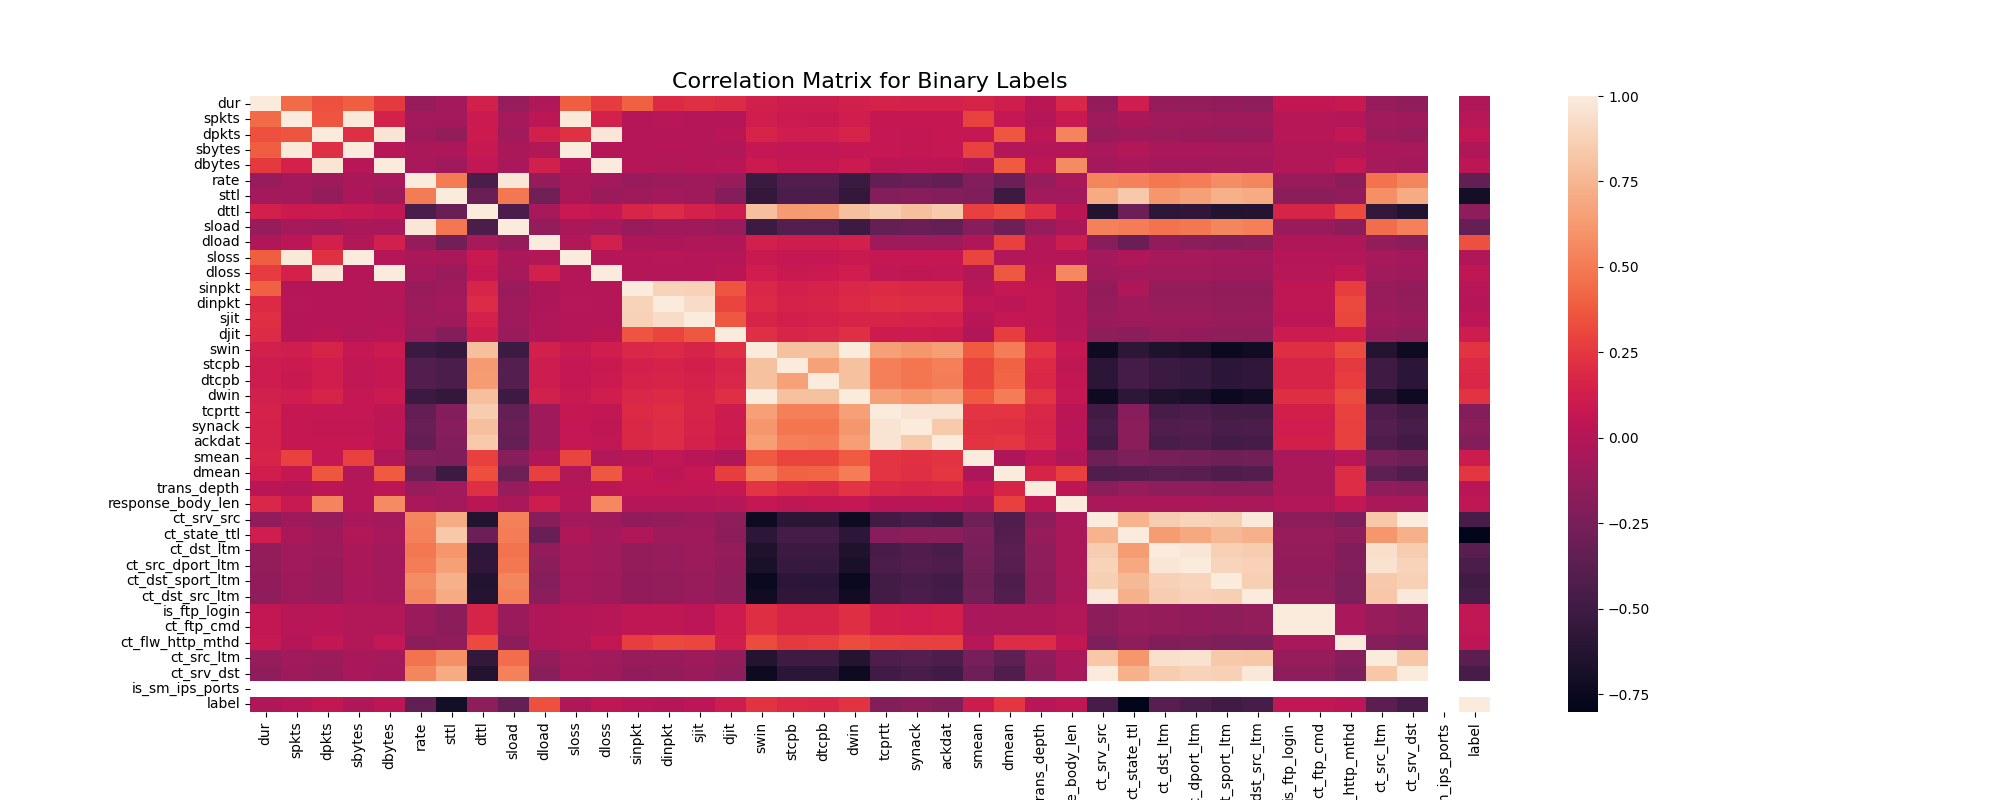
\includegraphics[width=4in,height=2in]{pic/correlation_matrix_bin.png}
\caption{Dataflow design}
\end{figure}



\newpage
\section{Use case Diagram}
use cases represent the main functionalities and tasks involved in the audio visual speech separation system. Each use case contributes to the overall process of capturing, processing, integrating, separating, and post-processing the audio and visual data to achieve the desired outcome of individual speech signal separation.
\begin{description}
    \item [Pre-process Audio:] This use case involves pre-processing the captured audio data. It may include operations like filtering, noise reduction, and echo cancellation to improve the quality of the audio signals.

\item [Process Visual:] This use case involves processing the captured visual data. It includes tasks such as face detection, facial landmark tracking, or lip motion analysis to extract relevant visual cues associated with speech production.

\item [Integrate Audio-Visual:] This use case represents the integration of the pre-processed audio data and processed visual data to create a synchronized audio-visual representation, aligning the audio and visual streams.

\item [Extract Features:] This use case involves extracting relevant features from the integrated audio-visual representation. It may include computing spectrograms, MFCCs, facial landmarks, or other visual and audio features.

\item [Perform Speech Separation:] This use case focuses on the actual speech separation process. It utilizes the extracted audio and visual features to separate the individual speech signals from the mixture, using techniques such as blind source separation or deep learning-based models.

\end{description}

\begin{figure}[hbtp]
\centering
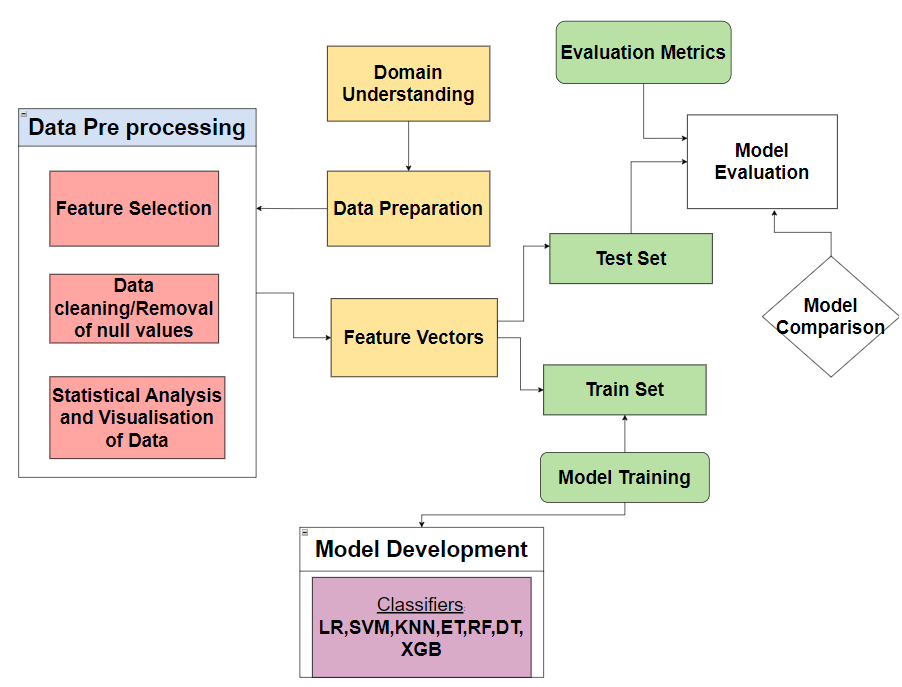
\includegraphics[width=9in,height=5in]{pic/flowchart.png}
\caption{Use case diagram for customer}
\end{figure}


\chapter{Implementation}


\section{Audio Extraction}
\par
Audio extraction is the process of isolating and extracting the audio content from a multimedia source, such as a video file. It involves separating the audio track from the accompanying video or other elements to obtain a standalone audio file representing the sound present in the source material.

\begin{figure}[hbtp]
\centering

\includegraphics[width=5in,height=3in]{./pic/sjeclogo.png}
\caption{code snippet for audio extraction}
\end{figure}

\section{Speech Separation}
\par SpeechBrain is an open-source framework 

\subsection{Sepformer}
\par SepFormer is an algorithm for speech separation that utilizes self-attention mechanisms. It employs a transformer-based architecture to capture long-range dependencies and model the relationships between time-frequency points in the audio mixture, enabling the separation of multiple speech sources from the mixture.


\begin{figure}[hbtp]
\centering

\includegraphics[width=5in,height=3in]{./pic/sjeclogo.png}
\caption{code snippet for speech separation}
\end{figure}

\section{Speech Enhancement}
\subsection{Lite Audio Visual Speech Enhancement}
\par
Lite AVSE algorithm is used for the separation and enhancement of the speech. The system 
includes two visual data compression techniques and removes the visual feature extraction 
network from the training model, yielding better online computation efficiency. As for the audio 
features, short-time Fourier transform (STFT) is calculated of 3-second audio segments. Each 
time-frequency (TF) bin contains the real and imaginary parts of a complex number, both of 
which used as input. Power-law compression used to prevent loud audio from overwhelming soft 
audio. The same processing is applied to both the noisy signal and the clean reference signal.

\begin{figure}[hbtp]
\centering
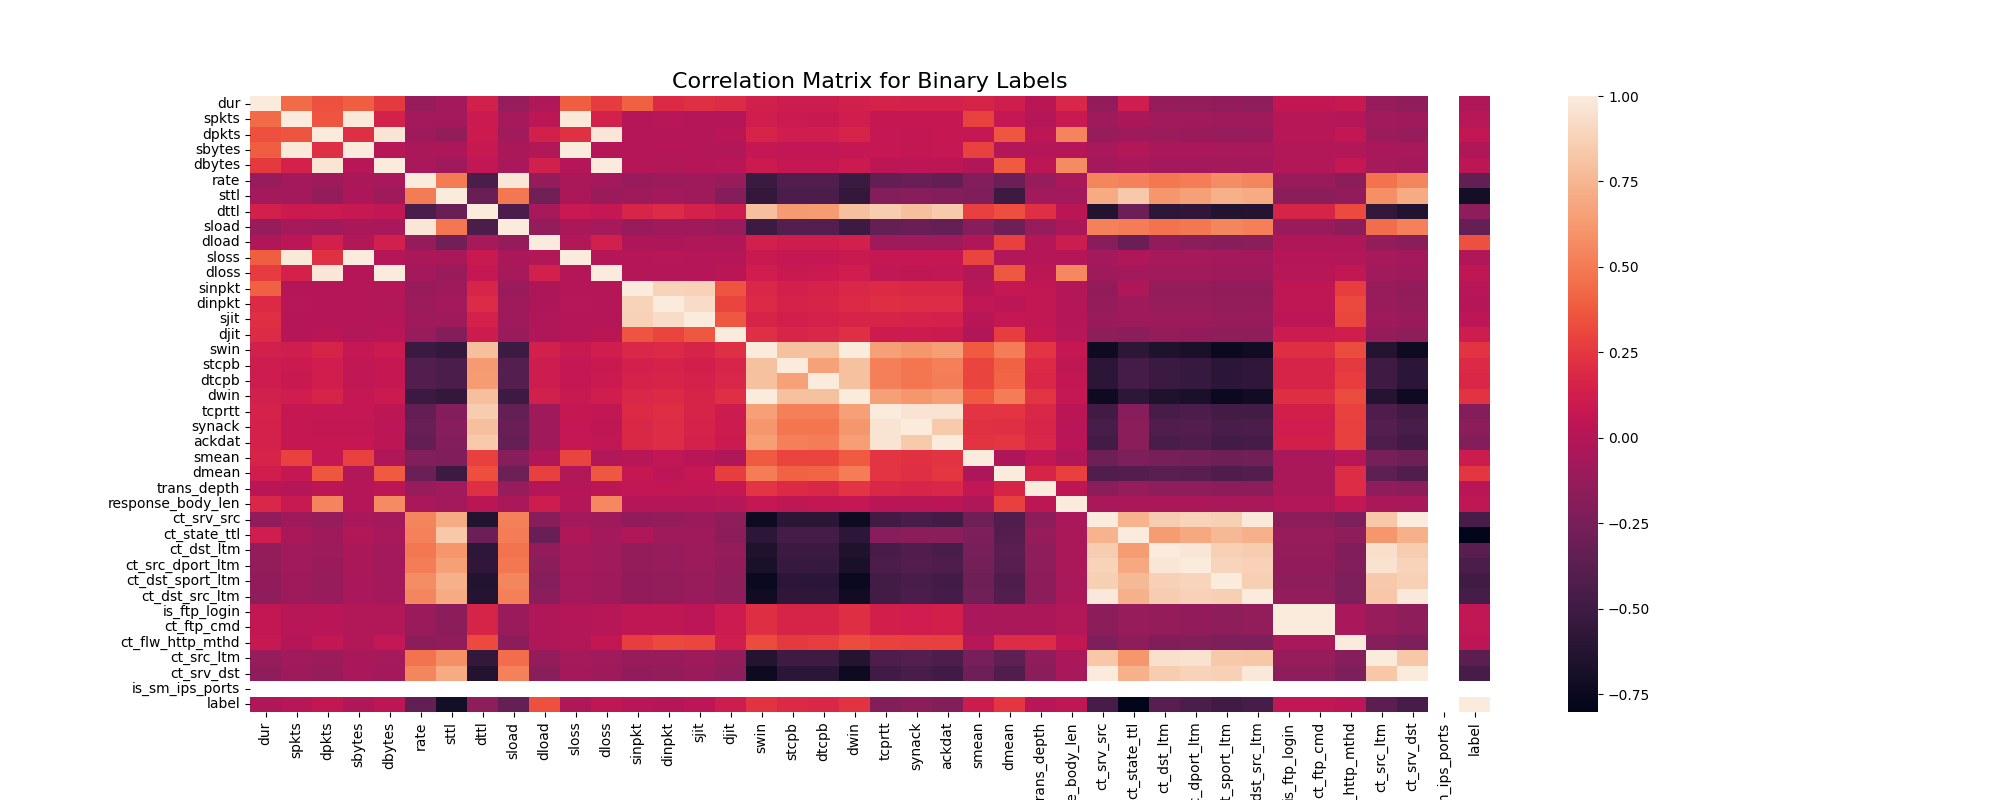
\includegraphics[width=5in,height=3in]{pic/correlation_matrix_bin.png}
\caption{code snippet for speech enhancement using LAVSE}
\end{figure}

\subsection{Spectral Subtraction}
Spectral subtraction is a technique used in audio signal processing to reduce background noise from an audio signal. It involves estimating the noise spectrum from a noisy signal and subtracting it from the noisy spectrum to enhance the desired signal. The resulting spectrum is then transformed back into the time domain to obtain a cleaner audio signal as in Figure \ref{fig:pic3}
\newpage
\begin{figure}[hbtp]
\centering

\includegraphics[width=5in,height=3in]{pic/sjeclogo.png}
\caption{code snippet for speech enhancement using spectral subtraction}
\label{fig:pic3}
\end{figure}

\section{Speaker Detection}
\par The cv2 functions provide methods to load the pre-trained models, apply them to images or video frames, and draw bounding boxes around the detected faces. By leveraging cv2's face detection capabilities, you can automate tasks such as facial recognition, emotion analysis, or face tracking in various applications like surveillance, biometrics, or augmented reality.


\begin{figure}[hbtp]
\centering
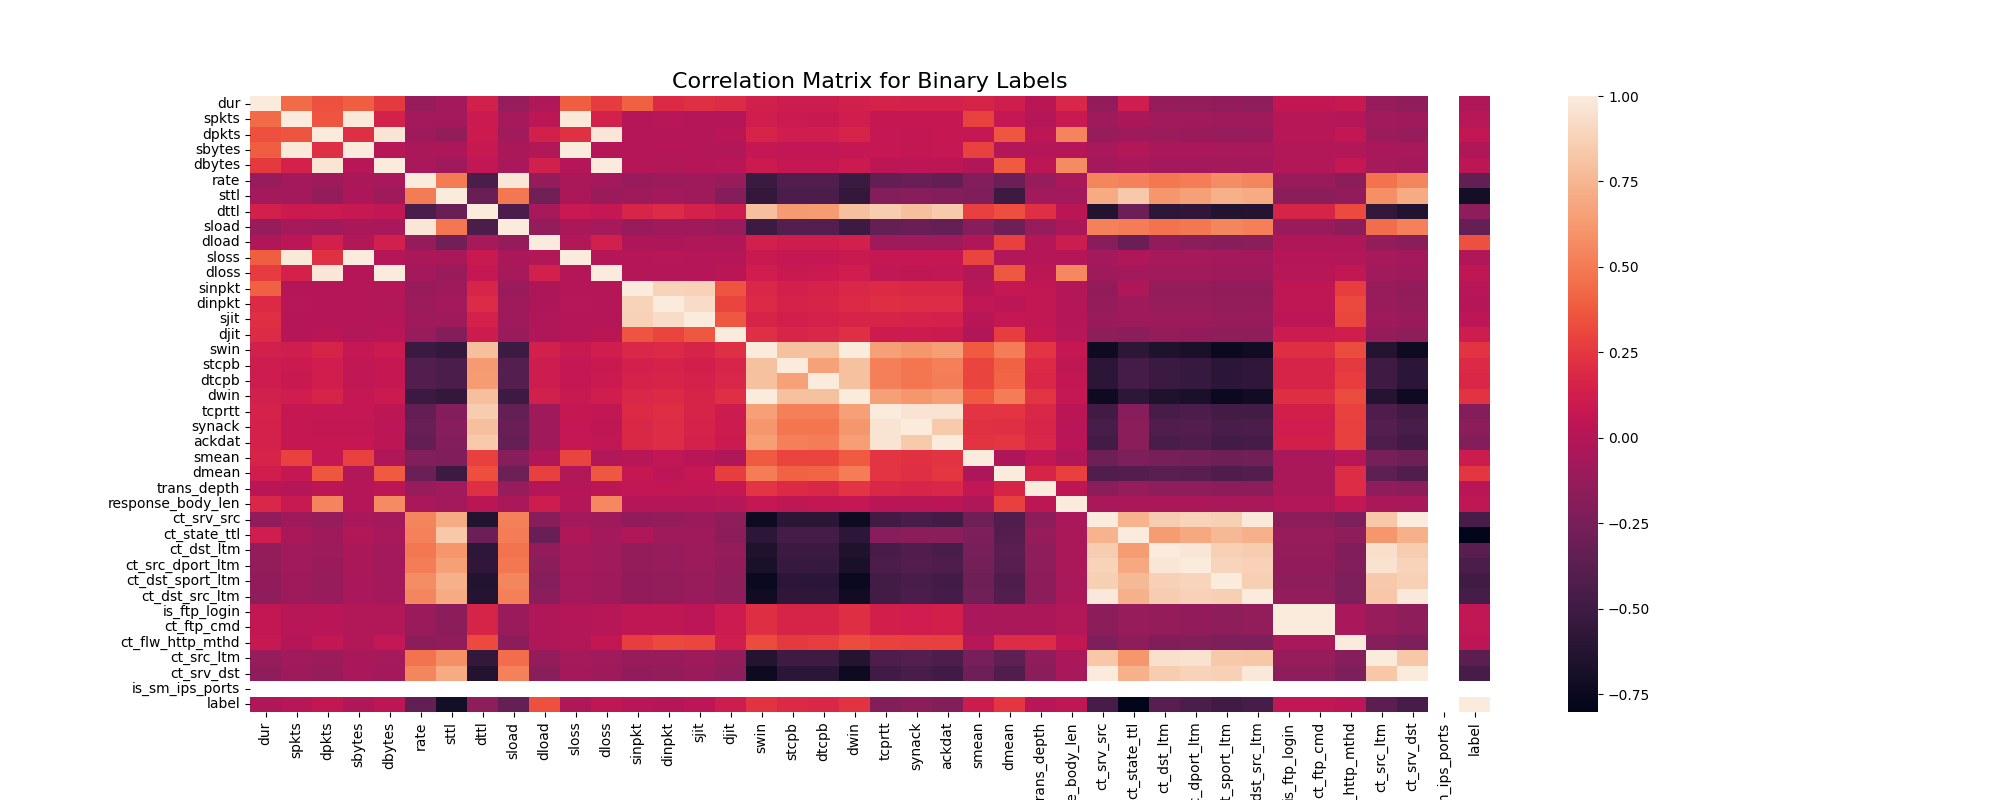
\includegraphics[width=5in,height=3in]{pic/correlation_matrix_bin.png}
\caption{code snippet for speaker detection}
\end{figure}





\chapter{System Testing}
\par
Testing is a procedure of executing the program with unequivocal intension of \cite{ref4}
discovering mistakes, assuming any, which makes the program, fall flat. This stage is an
essential piece of improvement.
\par
It plays out an exceptionally basic part for quality affirmation and for guaranteeing
unwavering quality of programming. It is the way toward finding the mistakes and
missing operation and furthermore an entire confirmation to decide if the targets are met
the client prerequisites are fulfilled.
\par
The objective of testing is to reveal prerequisites, outline or coding blunders in the
projects. Therefore, unique levels of testing are utilized in programming frameworks. The
testing results are utilized amid upkeep. The testcases are shown in Figure \ref{fig:pic4}

\section{Testing Objectives}
This area manages the points of interest in the various classes of the test which should be
directed to approve capacities, imperatives and execution. This can be accomplished
fundamentally by using the methods for testing, which assumes a crucial part in the
improvement of a product.

\section{Types of Testing conducted}
The structure of the program is not being considered in useful testing. Test cases are
exclusively chosen on the premise of the prerequisites or particulars of a program or
module of program but the internals of the module or the program are not considered for
determination of experiments\cite{ref1}.

\begin{figure}[h!]
\centering

\includegraphics[width=4in,height=1in]{pic/sjeclogo.png}
\caption{testcases}
\label{fig:pic4}
\end{figure}
The program to be tried is executed with an arrangement of experiments and the yield of
the program for the experiments is assessed to decide whether the program is executing
not surprisingly. The accomplishment of testing in uncovering mistakes in projects
depends basically on the experiments. There are two fundamental ways to deal with
testing Black Box or functional Testing and White Box or structural testing. Table \ref{tab:t1} shows the workflow. 
\begin{table} [htb]
\caption {Work Flow}
\vspace{0.25in}
\begin{tabular}{|c|c|c|}\hline
\textbf{Sl No}& \textbf{Work} & \textbf{Duration(in Weeks)}\\[6pt] \hline \normalsize
1&Audio Extraction&1 \\ \hline
2&Audio Enhancement using LAVSE&4\\ \hline
3&Audio Separation using Speechbrain&3\\ \hline
4&Noice Reduction using spectral subtraction&2\\ \hline
5&Image segmentation&3\\ \hline
6&Speaker Identification&5\\ \hline
\end{tabular}
\label{tab:t1}
\end{table}



\chapter{Results and Discussion}
\section{Face detection}
\begin{figure} [hbtp]
\centering

\includegraphics[width=5in,height=4in]{pic/sjeclogo.png}
\caption{Face detection}
\label{fig:pic5}
\end{figure}
\par Above Figure \ref{fig:pic5} shows initial face detection process using opencv and dlib. It convert the image to grayscale, apply the model using cv2.detectMultiScale(), and draw bounding boxes around the detected faces using cv2.rectangle(). Display or save the result using cv2.imshow() or cv2.imwrite().

\section{Speaker recognition}
\begin{figure} [hbtp]
\centering
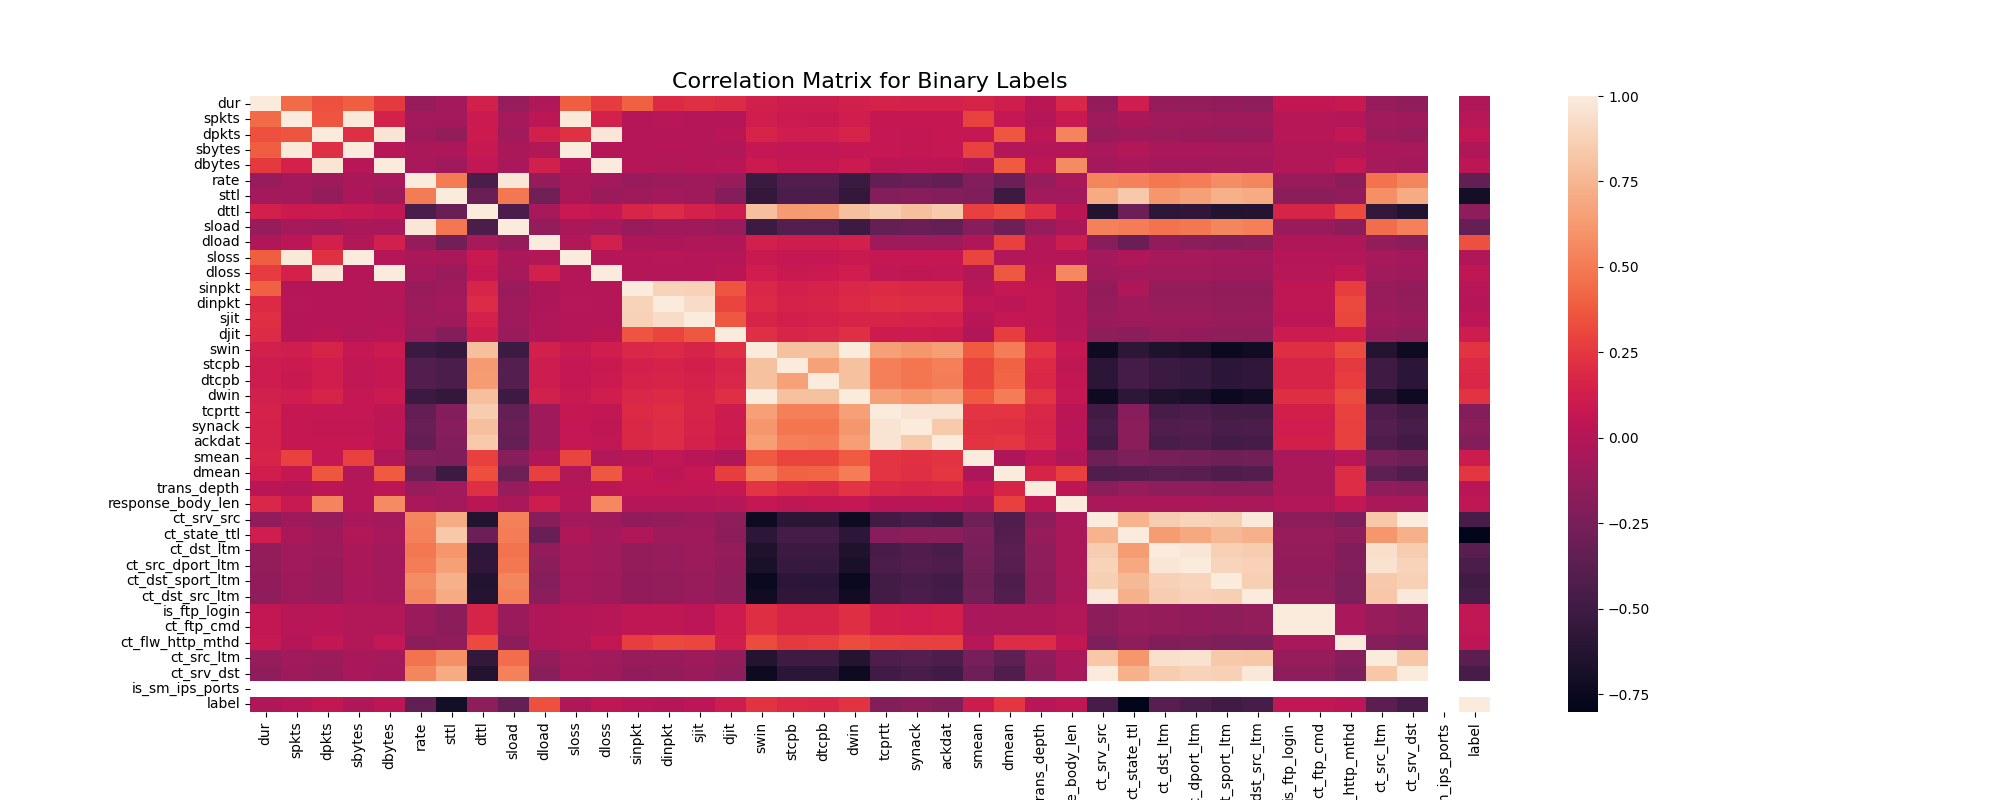
\includegraphics[width=5in,height=3in]{pic/correlation_matrix_bin.png}
\caption{Speaker recognition 1,person 1}
\end{figure}

\begin{figure} [hbtp]
\centering
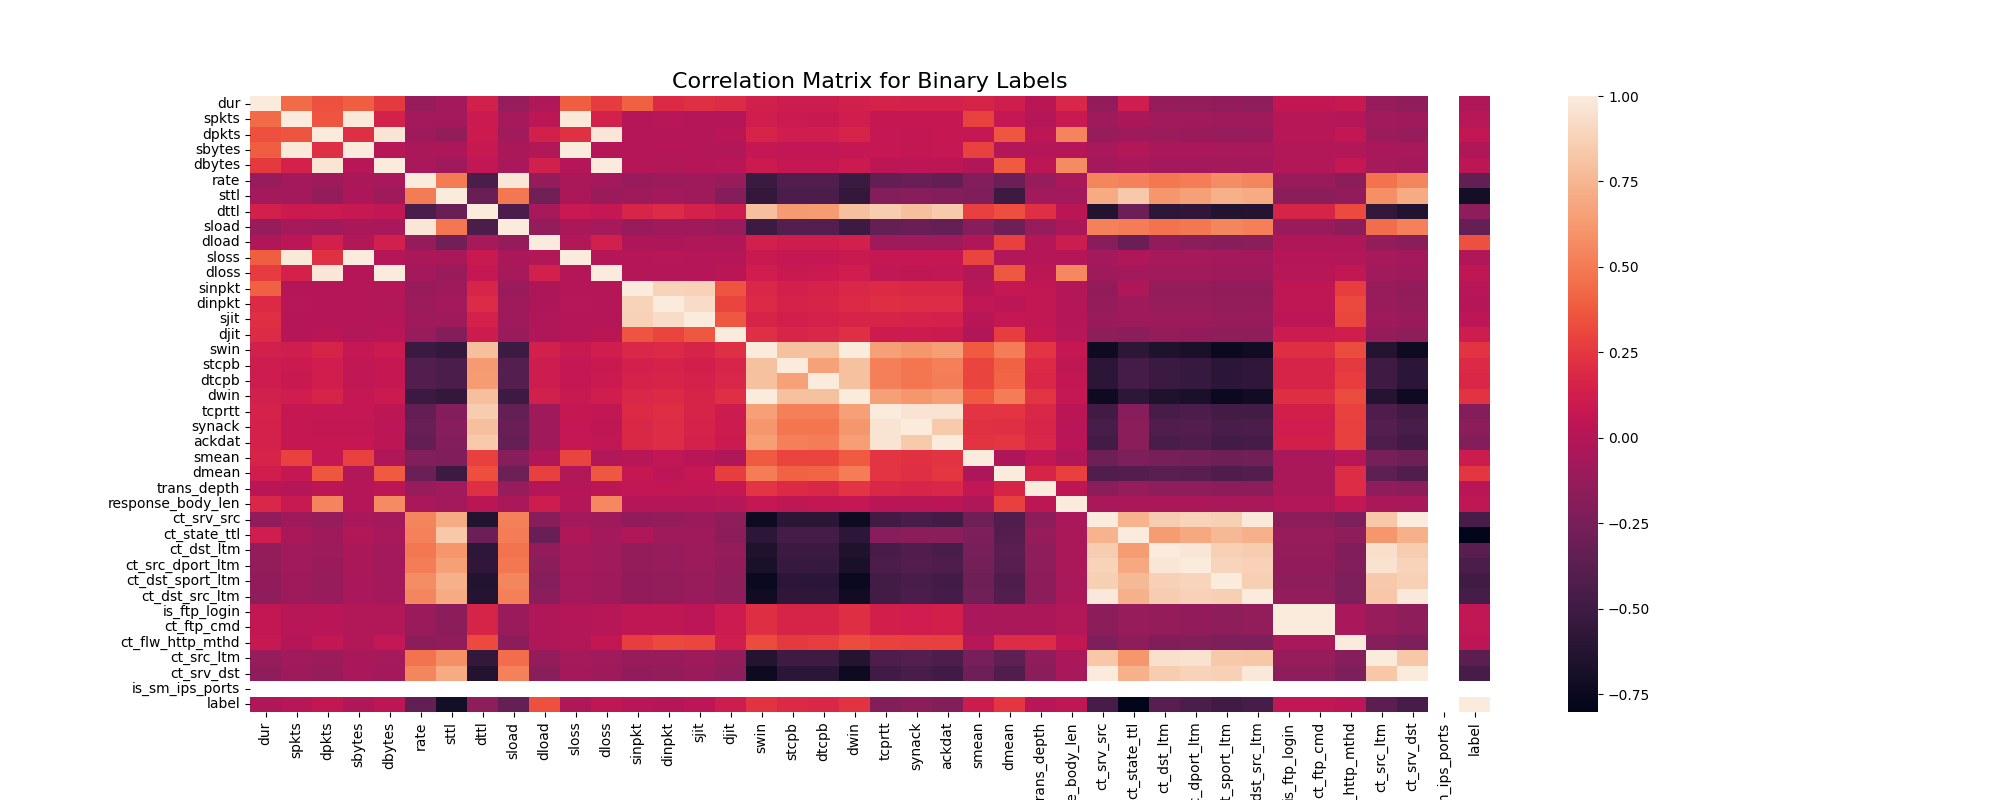
\includegraphics[width=5in,height=3in]{pic/correlation_matrix_bin.png}
\caption{Speaker recognition 1,person 2}
\end{figure}

\begin{figure} [hbtp]
\centering
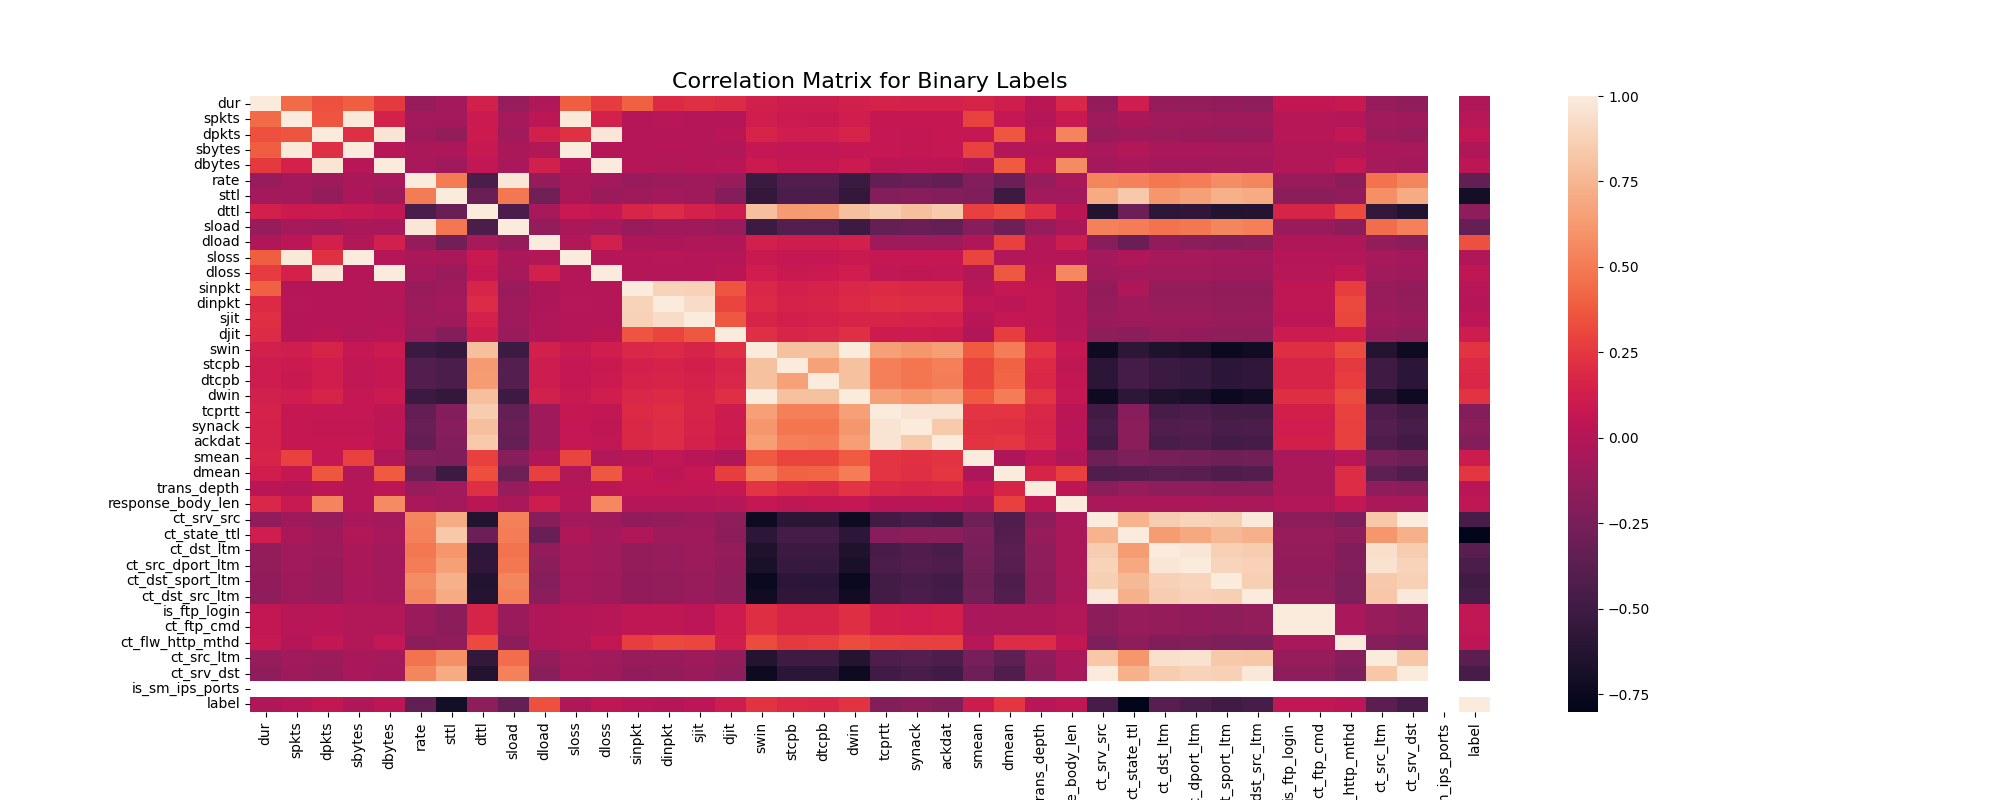
\includegraphics[width=5in,height=3in]{pic/correlation_matrix_bin.png}
\caption{Speaker recognition 2,person 1}
\end{figure}

\begin{figure} [hbtp]
\centering
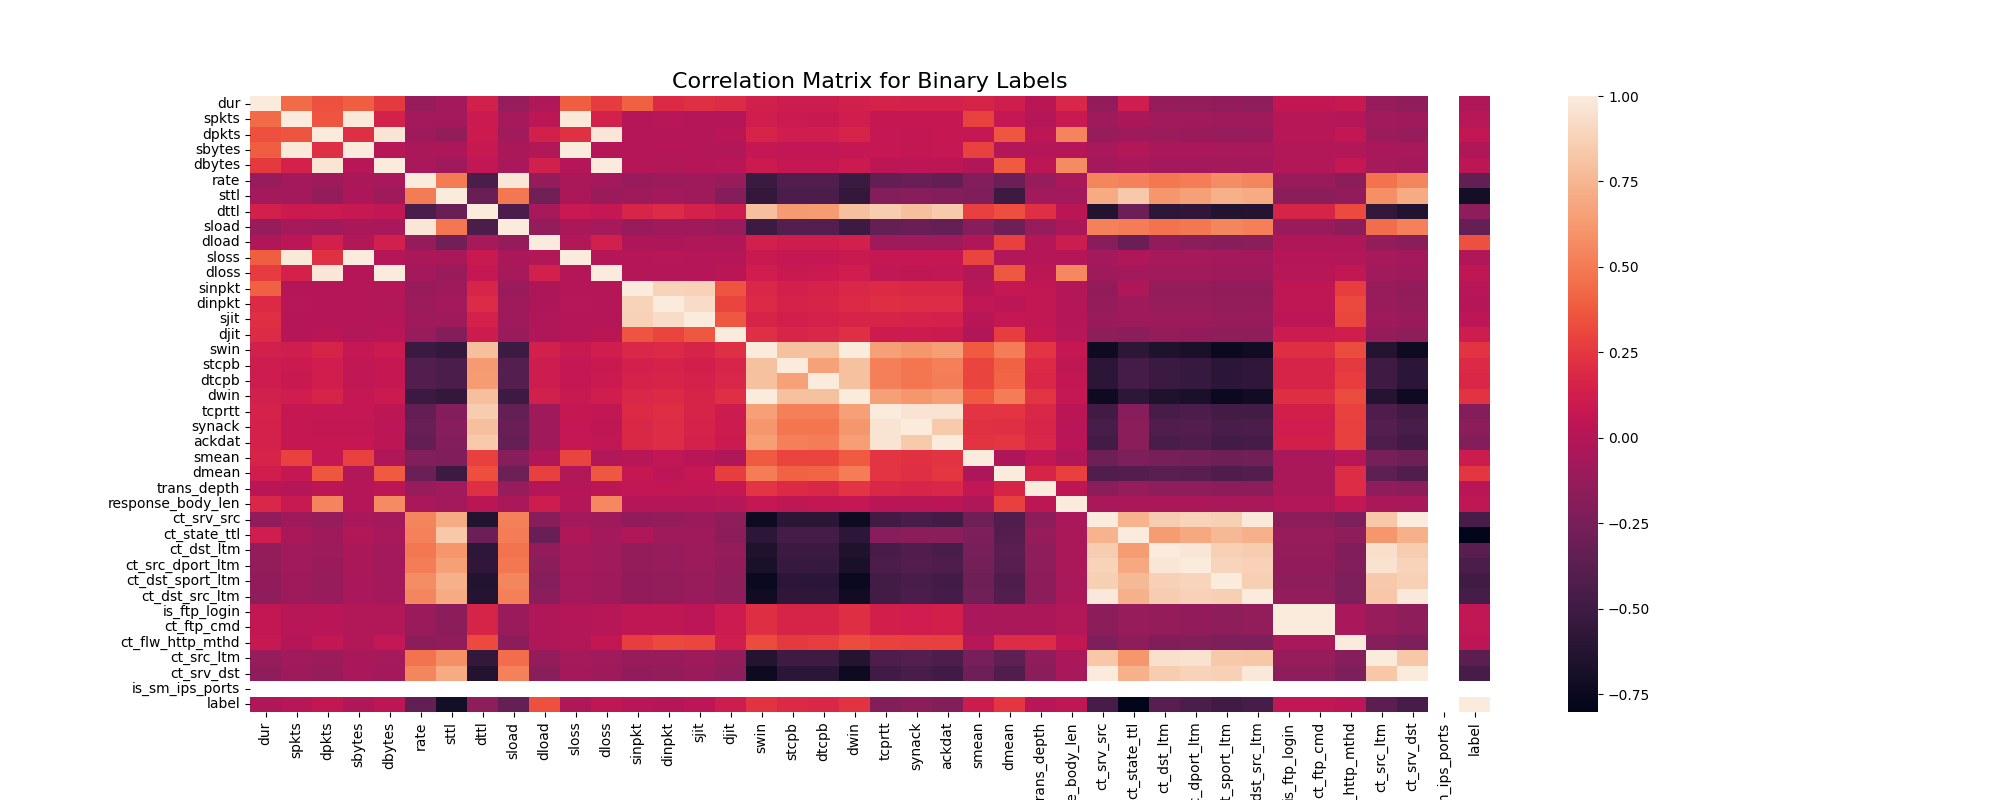
\includegraphics[width=5in,height=3in]{pic/correlation_matrix_bin.png}
\caption{Speaker recognition 2,person 2}
\end{figure}

\begin{figure} [hbtp]
\centering
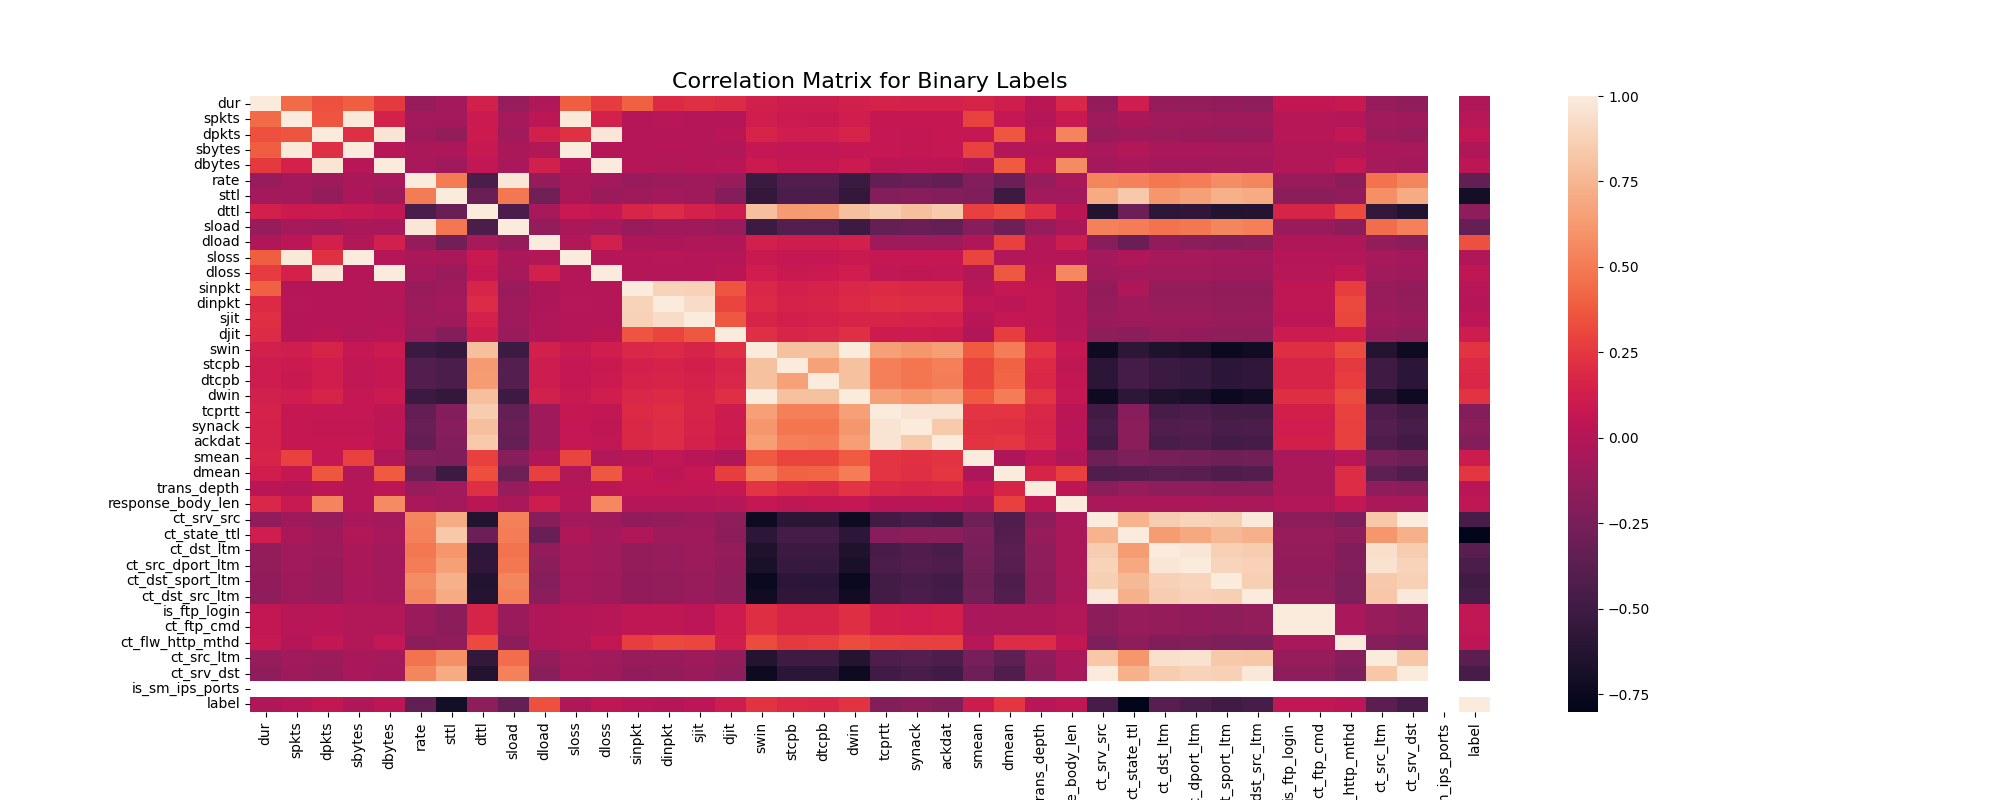
\includegraphics[width=5in,height=3in]{pic/correlation_matrix_bin.png}
\caption{Speaker recognition 3,person 1}
\end{figure}

\begin{figure} [hbtp]
\centering
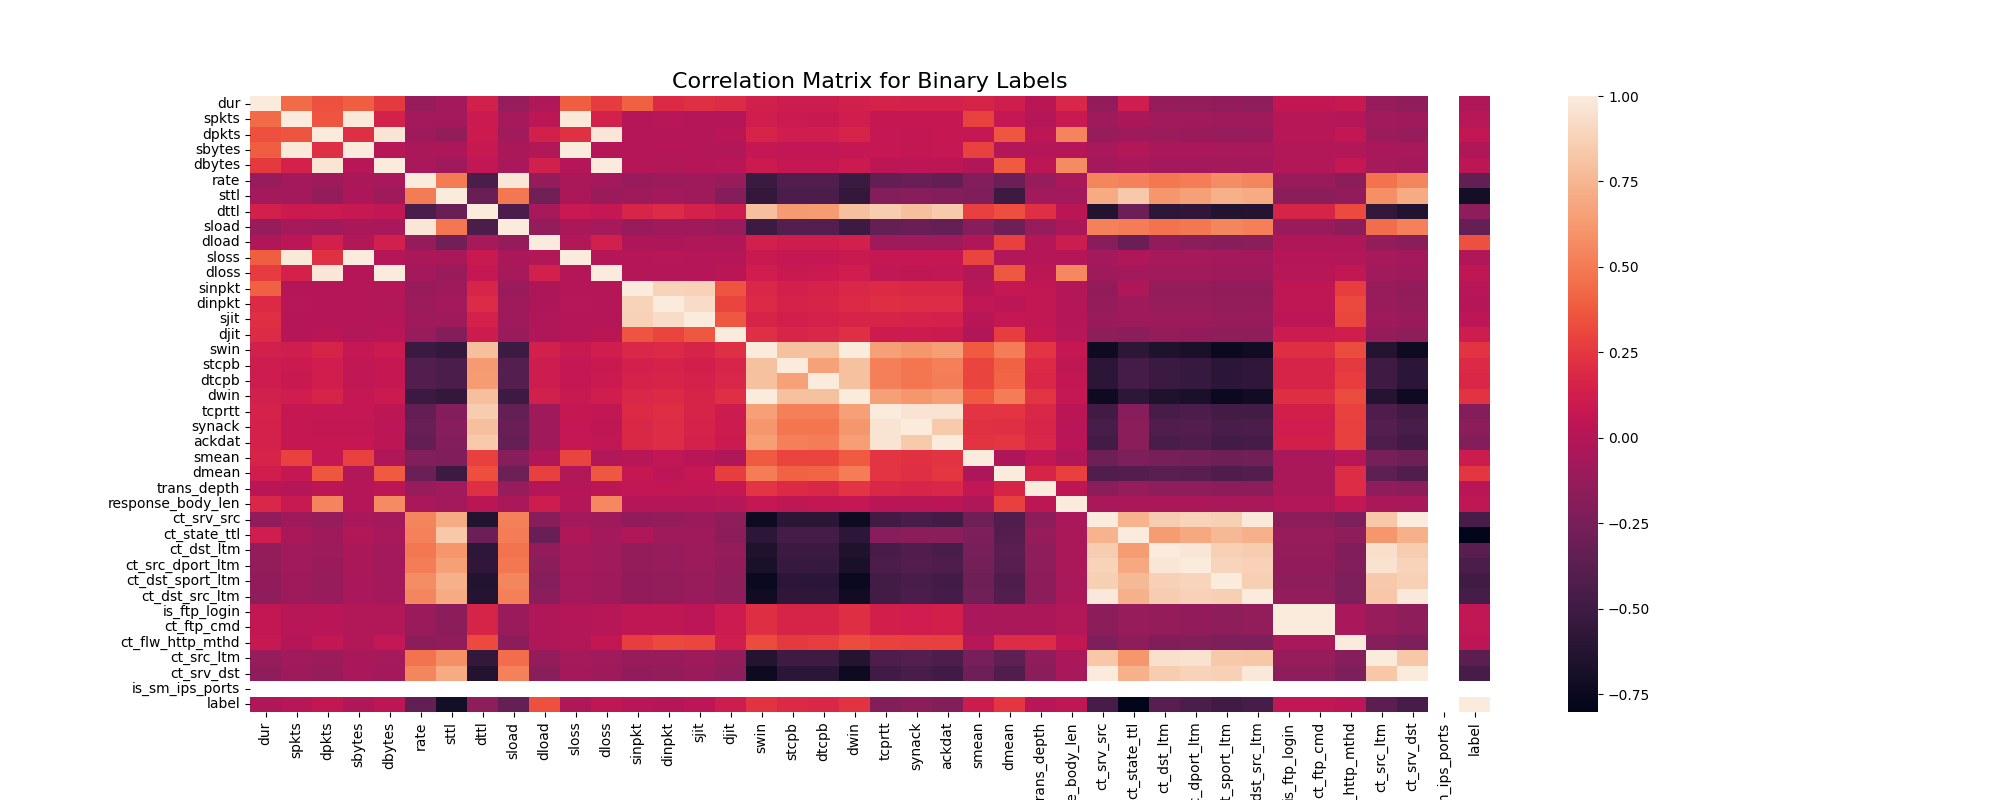
\includegraphics[width=5in,height=3in]{pic/correlation_matrix_bin.png}
\caption{Speaker recognition 3,person 2}
\end{figure}
\newpage
\par Above figures from 7.2 to 7.7 shows speaker recognition process using opencv and dlib.Speaker detection using cv2 and dlib involves utilizing dlib's pre-trained models along with cv2 functions to detect and locate human faces. By combining face detection with additional techniques such as audio analysis or lip movement tracking, speaker detection can be achieved in various applications like video conferencing or surveillance.

\chapter{Conclusion and Future work}
The Project will help in narrowing the imprecise communication problem in real-time data using 
speech separation and speaker identification technique by Deep Learning and Image Processing 
algorithms. This will impact the communication and security sectors in a greater extent. Overall, this 
project aims to develop an application or method that can help to separate the audio-visual speech and 
enhance it based on speaker identification.

\newpage
\pagestyle{plain}
\renewcommand{\bibname}{References}

\addcontentsline{toc}{chapter}{References}
% \begin{thebibliography}{35}
% \bibitem{ref1}
% Hu, G., Yang, Y., Yi, D., Kittler, J., Christmas, W.J., Li, S., \& Hospedales, T.M. "When Face Recognition Meets with Deep Learning: An Evaluation of Convolutional Neural Networks for Face Recognition," 2015 IEEE International Conference on Computer Vision Workshop (ICCVW), pp. 384–392, Dec. 2015, doi: 10.1109/iccvw.2015.58.

% \bibitem{ref2}
% Parkhi, Omkar, Andrea Vedaldi, and Andrew Zisserman. "Deep face recognition." In BMVC 2015-Proceedings of the British Machine Vision Conference 2015. British Machine Vision Association, 2015.

% \bibitem{ref3}
% Levitin, Anany. "Introduction to design and analysis of algorithms", 2/E. Pearson Education India, 2008.

% \bibitem{ref4}
% Prabhu, "Understanding of Convolutional Neural Network (CNN) — Deep Learning", URL: https://medium.com/\@RaghavPrabhu/understanding-of-convolutional-neural-network-cnn-deep-learning-99760835f148. Accessed on 23/07/2023

% \bibitem{ref5}
% L. Blanger and A. R. Panisson, “A Face Recognition Library using Convolutional Neural Networks,” International Journal of Engineering Research and Science, vol. 3, no. 8, pp. 84–92, Aug. 2017, doi: 10.25125/engineering-journal-ijoer-aug-2017-25.
% \bibitem{ref6}
% R. Khedgaonkar, K. Singh, and M. Raghuwanshi, “Local plastic surgery-based face recognition using convolutional neural networks,” Demystifying Big Data, Machine Learning, and Deep Learning for Healthcare Analytics, pp. 215–246, 2021, doi: 10.1016/b978-0-12-821633-0.00001-5.
% \bibitem{ref7}
% P. J. Phillips, “A Cross Benchmark Assessment of a Deep Convolutional Neural Network for Face Recognition,” 2017 12th IEEE International Conference on Automatic Face \&; Gesture Recognition (FG 2017), pp. 705–710, May 2017, doi: 10.1109/fg.2017.89.
% \bibitem{ref8}
% Z. Huang, J. Zhang, and H. Shan, “When Age-Invariant Face Recognition Meets Face Age Synthesis: A Multi-Task Learning Framework,” 2021 IEEE/CVF Conference on Computer Vision and Pattern Recognition (CVPR), pp. 7278–7287, Jun. 2021, doi: 10.1109/cvpr46437.2021.00720.
% \bibitem{ref9}
% Z. Huang, J. Zhang, and H. Shan, “When Age-Invariant Face Recognition Meets Face Age Synthesis: A Multi-Task Learning Framework,” 2021 IEEE/CVF Conference on Computer Vision and Pattern Recognition (CVPR), pp. 7278–7287, Jun. 2021, doi: 10.1109/cvpr46437.2021.00720.
% \end{thebibliography}

\printbibliography



\end{document}